\documentclass[final,3p,times,authoryear]{elsarticle}

\usepackage{amssymb}
\usepackage{amsmath}
\usepackage{graphicx}
\usepackage{booktabs}
\usepackage{longtable}
\usepackage{array}
\usepackage{hyperref}
\usepackage{url}

\journal{Risks}

\begin{document}

\begin{frontmatter}

\title{Extreme Commodity Tail Risk and Exchange-Rate Exposure in Ghana:
Copula--EVT Evidence from Cocoa, Gold, Oil and the Cedi}

\author{Jonathan Nelson}
\address{Independent Research Project}

\begin{abstract}
Commodity-dependent economies face two distinct risks: the economic risk
that export commodities crash together in a crisis, and the model risk
of measuring that exposure with dependence tools too narrow for the
data. Ghana is a natural setting to separate the two, since cocoa, gold
and crude oil together account for the large majority of its export
receipts. We build a copula--extreme-value-theory framework for daily
cocoa, gold, Brent and WTI returns and the Bank of Ghana's official
interbank USD/GHS rate, spanning 2015--2026, with adequacy-gated
marginal filtering, an eight-family copula stack screened by formal
goodness-of-fit testing, and moving-block bootstrap inference corrected
for sixty simultaneous hypothesis tests by both family-wise Bonferroni
and Benjamini--Hochberg false-discovery-rate methods. We find no robust
evidence that tail dependence among the three commodities intensifies
during stress -- tested separately for the COVID shock, the 2024 cocoa
supply crisis, and their combination -- and no detectable commodity-to-
cedi transmission channel at daily-to-monthly frequency. Model risk,
however, is substantial and economically important in its own right:
even after tripling the candidate copula families, six of ten pairs
reject every family tested, indicating real dependence whose shape
standard tools cannot capture, while the cedi's own extreme-value
profile is the heaviest tail in the panel and resists six independent
attempts at adequate marginal modelling, including an explicit
zero-inflated hurdle specification and a two-state Markov-switching
model. For risk management, this implies Ghana's commodity exposure
should not be assumed to intensify automatically in every crisis, but
that model risk in how that exposure is measured deserves as much
attention as the exposure itself.
\end{abstract}

\begin{keyword}
tail dependence \sep copulas \sep extreme value theory \sep model risk
\sep commodity risk \sep Ghana \sep exchange-rate exposure \sep stress
testing
\end{keyword}

\end{frontmatter}


\section{Introduction}
\label{sec:intro}

Commodity-dependent economies carry two distinct kinds of risk that are
easy to conflate. The first is economic: if the commodities that
dominate a country's export base crash together in a crisis, its
foreign-exchange and fiscal exposure is larger than any single-commodity
risk assessment implies. The second is a model risk, one step removed
from the first: even where genuine dependence exists, standard tools
for measuring it -- correlation, or a narrow, conveniently tractable set
of copula families -- may simply be the wrong shape for the data,
producing risk estimates that are precise but not accurate. A
commodity-dependent economy that manages the first risk without
attending to the second has not actually reduced its exposure; it has
only changed which risk is invisible to it.

Ghana is close to an ideal setting to study both risks together. Cocoa,
gold and crude oil jointly dominate its export receipts: using Bank of
Ghana merchandise trade data for 2022, gold accounted for 38.0\% of
merchandise exports (f.o.b.), crude oil 31.2\%, and cocoa beans and
cocoa products a combined 12.8\%, together well over 80\% of the total
--- a level of concentration in three commodity classes that few
economies of Ghana's size share. Extreme moves in any of the three
therefore have a direct line to the country's foreign-exchange position,
transmitted through export revenue, reserve accumulation, and the fiscal
channel via royalties and taxes on commodity production. Whether that
exposure is compounded by extreme commodity prices moving together, and
whether it shows up detectably in the exchange rate the central bank
manages, are risk-management questions with direct operational stakes,
not only an econometric curiosity.

We ask three questions. First, do cocoa, gold and crude oil exhibit
tail dependence -- co-movement concentrated specifically in extreme
outcomes, beyond what ordinary correlation would predict -- and does
that dependence intensify during periods of market stress? Second, is
that dependence, wherever it exists, adequately described by the
standard toolkit of parametric copula families, or does relying on that
toolkit itself constitute an unmeasured source of model risk? Third,
does joint commodity tail risk transmit into Ghana's exchange rate at a
frequency where it would actually be useful for monitoring purposes?

The third question requires an explicit caveat that shapes how we
interpret our own results. Commodity shocks can affect the cedi through
several channels -- export receipts, reserve buffers, the fiscal
position, and market expectations -- and none of these channels have an
obvious reason to operate at daily frequency. A central bank's reserve
response to a commodity shock, for instance, is a policy decision made
over weeks or months, not an automatic same-day market reaction. We
therefore test for transmission at both daily and monthly frequency and
are careful throughout to phrase any null result as an absence of
\emph{detectable} transmission within the frequency, sample period, and
model specification tested here, not as a claim that no such channel
exists at any frequency whatsoever.

The 2024 cocoa episode adds a further layer of interpretive care. Unlike
a classic joint crash, 2024 was an upper-tail event for cocoa: West
African supply failures drove prices to repeated all-time highs, while
gold and oil markets remained comparatively orderly. A price
\emph{surge} of this kind is not "bad" for Ghana as a producer in the
way a crash is -- higher cocoa prices raise export revenue -- so testing
this episode requires distinguishing upper-tail from lower-tail
dependence throughout, rather than treating "stress" as synonymous with
"crash," and requires testing 2024 both combined with, and separately
from, the COVID shock, since the two are different kinds of stress event
by any reasonable economic description.

Our contribution follows directly from these three questions. On the
economic-risk question, we provide a rigorously tested answer: no robust
evidence of stress-driven tail-dependence intensification among the
three commodities, corrected for the full sixty-cell space of pairs,
quantile levels and tails tested, by two independent multiple-testing
procedures that agree with each other. On the model-risk question, we
provide what we believe is a genuinely novel finding for this
literature: expanding the candidate copula set from four families to
eight -- adding Frank, Joe, and the rotated (survival) Clayton and
Gumbel families -- does not rescue the six pairs whose dependence
structure the narrower set already found impossible to fit; every
family, in all eight, is rejected by formal goodness-of-fit testing for
those six pairs. This is model risk made concrete and quantified, not
asserted. On data quality, we show that the Bank of Ghana's official
interbank rate and the free Yahoo Finance proxy commonly used in its
place diverge sharply in returns (correlating at only 0.18 once outright
data errors are excluded), and we subject the cedi's own difficult
managed-float marginal to six independent modelling treatments,
including an explicit hurdle model and a Markov-switching specification,
to establish that our substantive conclusions do not depend on which
treatment is chosen.

The remainder of the paper proceeds as follows. Section~\ref{sec:lit}
situates the paper in the copula, extreme-value and commodity-contagion
literatures. Section~\ref{sec:data} documents data construction.
Section~\ref{sec:methodology} sets out the full methodology.
Section~\ref{sec:results} reports the main findings.
Section~\ref{sec:robustness} summarizes robustness checks, with full
detail in the appendices. Section~\ref{sec:discussion} discusses
risk-management implications. Section~\ref{sec:limitations} states
limitations. Section~\ref{sec:conclusion} concludes.

\section{Related literature}
\label{sec:lit}

Three strands of literature inform this paper.

The copula and tail-dependence literature establishes that dependence
beyond correlation is captured by the copula function, and that copula
families differ sharply in tail behaviour. Sklar's theorem
\citep{sklar1959} underlies the two-step estimation strategy used
throughout. Joe \citep{joe1997} and Nelsen \citep{nelsen2006} set out
the standard taxonomy: the Gaussian copula is asymptotically
tail-independent at any correlation below one; the Student-$t$ copula is
tail-dependent and symmetric; the Clayton and Gumbel families are
tail-asymmetric, concentrating dependence in the lower or upper tail
respectively. McNeil, Frey and Embrechts \citep{mcneil2015} provide the
quantitative risk management context this paper operates in. Hua and
Joe \citep{hua2011} distinguish intermediate from asymptotic tail
dependence via the behaviour of the empirical tail-concentration
function as the quantile shrinks, the interpretive frame we use
throughout for our own $q$-indexed estimator. Genest, Ghoudi and Rivest
\citep{genest1995} establish the semiparametric pseudo-maximum-likelihood
approach this paper's copula stage relies on, and Genest, R\'emillard
and Beaudoin \citep{genest2009} develop the Rosenblatt-transform
Cram\'er--von Mises goodness-of-fit test with parametric bootstrap that
this paper uses as its formal arbiter of copula adequacy -- a step we
extend here to a substantially wider family set than is typical in
applied tail-dependence work.

The extreme-value strand motivates our treatment of each series' own
tail. The Pickands--Balkema--de Haan theorem \citep{balkema1974,pickands1975}
justifies peaks-over-threshold GPD fitting; Embrechts, Kl\"uppelberg and
Mikosch \citep{embrechts1997} provide the comprehensive extremal-event
treatment this paper draws on; McNeil and Frey \citep{mcneil2000}
establish the two-step GARCH-EVT construction this paper's marginal
stage implements.

The commodity-contagion and financialization literature documents rising
cross-commodity co-movement and its transmission into commodity-dependent
currencies. Tang and Xiong \citep{tang2012} document
financialization-driven increases in cross-commodity correlation, the
concern this paper tests directly. Silvennoinen and Thorp
\citep{silvennoinen2013} document time-varying dependence across
commodity futures. Reboredo \citep{reboredo2012} applies copula methods
to oil-exchange-rate co-movement, the closest methodological precedent
to our commodity-cedi analysis. Cocoa, with its distinctive West African
supply geography and a 2024 price episode without close historical
precedent in our sample, remains comparatively understudied relative to
oil and metals in this literature.

\section{Data}
\label{sec:data}

The daily layer comprises ICE cocoa, COMEX gold, Brent and WTI crude
futures from Yahoo Finance, and the Bank of Ghana (BoG) interbank
USD/GHS mid-rate, January 2015 through July 2026, in continuously
compounded percentage returns. Yahoo's terms of service permit research
use of this data but prohibit redistribution; our fetch code, not the
raw files, is what we make public. Yahoo's continuous-futures series are
front-month contracts rolled without back-adjustment, so daily returns
contain mechanical roll jumps that are not distinguishable from genuine
price moves within the series alone; we address this directly in
Section~\ref{sec:robustness} via an independent monthly benchmark. One
cleaning step affects every commodity series identically: the 20 April
2020 negative WTI settlement, an artifact of that contract's physical-
delivery mechanics during an unprecedented storage crisis, is masked
(its log return is undefined) rather than silently dropped or imputed.

\subsection{The cedi series}
\label{sec:cedi-provenance}

We use the official BoG interbank USD/GHS mid-rate as the cedi series in
place of the free Yahoo Finance proxy (ticker GHS=X) commonly used for
this purpose, a choice with material consequences we document rather
than assert. Over the 2,850-day overlap, the two series' \emph{levels}
agree closely once two outright Yahoo data errors are excluded (level
correlation 0.997) -- a 573.00 print on 2020-03-31 against BoG's 5.44,
and a 1.00 print on 2016-05-13 against BoG's 3.81 -- but their
\emph{returns} correlate at only 0.18 even after excluding those errors.
Since tail-dependence estimation is a statement about the joint
distribution of returns, not levels, this gap is decisive: Yahoo's feed
is dominated by stale, infrequently updated quotes punctuated by
occasional large catch-up jumps, exactly the pattern that would corrupt
a tail analysis. The December 2022 debt-restructuring episode
illustrates the practical difference: the BoG series records a smooth
appreciation from 12.90 (8 December) to 8.00 (15 December), coinciding
with Ghana's IMF staff-level agreement, while Yahoo sits stale near 11.8
through the same window and then registers a single artificial jump on
16 December. A three-day-window adjudication procedure confirms this
directly: of three dates initially flagged as suspect disagreements, two
resolve as pure Yahoo artifacts with no comparable BoG move, and the
December 2022 date resolves as a genuine BoG move, correctly present in
the BoG series on its true dates and retained without alteration. No
automatic bad-tick filter is applied to the BoG series itself, consistent
with treating it as the official reference: every large move in it is
treated as real by construction.

The cedi series carries a structural feature central to everything that
follows: as a managed float, 22.3\% of its daily returns are exactly
zero and a further 12.7\% of the remaining nonzero returns lie within
0.5\% in magnitude, consistent with long stretches of administered
stability interrupted by occasional large adjustments. All five return
series are oriented so the lower tail denotes an outcome adverse to
Ghana; since the cedi is quoted as GHS per USD, its return series is
sign-flipped so that depreciation, like a commodity price crash, falls
in the lower tail.

\subsection{Ghana macroeconomic data}
\label{sec:macro-data}

The transmission analysis in Section~\ref{sec:results} uses monthly
Bank of Ghana series: headline year-on-year CPI inflation (108
observations, January 2015 to December 2023, within our analysis
window) and merchandise exports, f.o.b. (100 observations, January 2015
to April 2023). Constructing the exports series required correcting a
data-extraction error we describe in full, with its resolution, in
Appendix~\ref{app:decisions}: the underlying BoG table stacks eight
distinct series -- total exports, the trade balance, and six commodity
sub-components -- under a single value column, and an unfiltered
extraction silently mixed the (legitimately negative) trade balance into
what should have been a pure export level; a second, independent issue
in the same table encodes an eight-month reporting gap as a literal
value of zero rather than a missing-data marker. Both are corrected and
verified directly against the raw source in Appendix~\ref{app:decisions}.

\section{Methodology}
\label{sec:methodology}

\subsection{Marginal models}
\label{sec:marginals}

Each return series is filtered through a conditional mean-and-variance
model before any dependence structure is estimated. Rather than fixing
one specification, each series is passed through an adequacy-gated
ladder: an AR(1)-GJR-GARCH(1,1)-$t$ baseline \citep{bollerslev1986,glosten1993}
is checked against three diagnostics -- Ljung--Box on standardized
residuals and on their squares, and a Kolmogorov--Smirnov test of PIT
uniformity -- and, if any fails at 5\%, the series is refit under an
AR(2) mean, an EGARCH(1,1) variance \citep{nelson1991}, and a GJR-GARCH
with skew-$t$ innovations, in that order, stopping at the first
specification passing all three tests. If none passes, the lowest-AIC
specification is retained and the failure disclosed. Standardized
residuals are mapped to pseudo-uniform observations by the probability
integral transform under the fitted innovation distribution, then
re-ranked into pseudo-observations, isolating any residual
misspecification to the marginal stage \citep{genest1995,joe2005}.

\subsection{Extreme value margins}

The loss tail of each standardized-residual series is fit by
peaks-over-threshold: exceedances of the 90th-percentile threshold are
fit with a generalized Pareto distribution, justified asymptotically by
the Pickands--Balkema--de Haan theorem \citep{balkema1974,pickands1975}.
Threshold sensitivity is scanned from the 85th to 97.5th percentile for
every series; block-maxima GEV fits provide an independent cross-check
resting on a different asymptotic theorem (Fisher--Tippett--Gnedenko)
and a different data-reduction strategy.

\subsection{Copulas, tail dependence, and goodness-of-fit}
\label{sec:copula-method}

For each of the ten series pairs we estimate copulas by pseudo-maximum
likelihood on the rank-based pseudo-observations. Beyond the four
families conventionally used in applied tail-dependence work --
Gaussian (tail-independent benchmark), Student-$t$ (symmetric tail
dependence), Clayton (lower-tail only) and Gumbel (upper-tail only) --
we add four further families to test directly whether a narrow
candidate set is itself a source of model risk: Frank (no tail
dependence, flexible symmetric mid-range dependence), Joe (upper-tail
dependence of a different functional shape than Gumbel), and the
survival (180-degree rotated) Clayton and Gumbel copulas, which invert
which tail carries the asymmetric dependence. Model selection among all
eight is by AIC.

Because AIC selects the best-fitting family \emph{among the candidates}
but says nothing about absolute adequacy, every fitted family for every
pair is subjected to the Rosenblatt-transform Cram\'er--von Mises
goodness-of-fit test of \citet{genest2009}: the fitted copula's
Rosenblatt transform should, under correct specification, itself be
independent-uniform on the unit square, and a parametric bootstrap (500
replicates per family per pair, 4,000 replicates total) provides the
null reference distribution against which the observed statistic is
compared. A family is judged not rejected at 5\% if its statistic falls
below the bootstrap's 95th percentile.

Independently of any fitted family, a nonparametric empirical
tail-concentration estimator is computed at $q \in \{0.025, 0.05,
0.10\}$ in both tails,
$\hat\lambda_L(q) = \#\{u_i \le q, v_i \le q\}/(nq)$ and its upper-tail
analogue, interpreted throughout as a statement about concentration at
the tested quantile rather than a direct estimate of the asymptotic
coefficient, following \citet{hua2011}.

\subsection{Stress-versus-calm inference and multiple-testing correction}
\label{sec:inference-method}

Two stress windows are fixed \emph{ex ante}: the COVID shock (March--June
2020) and the 2024 cocoa shock (calendar 2024). Both are tested three
ways -- combined, and each separately against a calm baseline held
constant across all three comparisons (excluding both windows throughout,
so that a difference between the COVID-only and 2024-only results
reflects which episode drives any signal, not a shifting comparison
group) -- since the two episodes are different kinds of stress by any
reasonable economic description: COVID a broad-based crash-type shock,
2024 a cocoa-specific supply-driven price surge.

Significance of the calm-versus-stress difference in $\hat\lambda(q)$ is
assessed by a moving-block bootstrap \citep{kunsch1989} (block length 20
trading days, 500 replicates as a baseline, increased to 15,000 for any
cell whose bootstrap resolution proves insufficient at the correction
level required -- a diagnostic check applied systematically rather than
left to chance, since a coarse bootstrap can produce a spuriously round,
apparently-significant $p$-value that is actually an artifact of too few
replicates to resolve a stringent threshold). Across the full sweep of
ten pairs, three quantile levels and two tails, sixty simultaneous tests
are conducted per stress-window definition. We report significance under
three criteria: uncorrected (5\%), a family-wise Bonferroni correction
across all sixty cells simultaneously ($\alpha/60$), and a
Benjamini--Hochberg false-discovery-rate procedure at 5\% across the
same sixty $p$-values. Reporting both corrections is deliberate: they
rest on different assumptions, and a result surviving only one is weaker
evidence than a result neither touches, or than a null conclusion both
agree on.

\subsection{Roll-effect validation}
\label{sec:pinksheet-method}

Because Yahoo's futures series are unadjusted for contract rolls, we
validate the daily return series against an independent, non-futures
benchmark: the World Bank's Commodity Price Data (``Pink Sheet''),
which reports monthly average prices for cocoa, gold, Brent and WTI from
underlying reference prices rather than a rolled futures contract. The
comparison requires matching sampling conventions precisely: the Pink
Sheet's documented methodology is a monthly \emph{average}, so Yahoo's
daily series is resampled to its own monthly mean for comparison, not an
end-of-month snapshot, which would conflate a genuine roll-effect
question with an unrelated sampling-convention mismatch.

\subsection{Cedi marginal robustness}
\label{sec:cedi-robustness-method}

Given the cedi's structural difficulty (Section~\ref{sec:cedi-provenance}),
we test whether our substantive conclusions depend on how its marginal
is treated, across six independent constructions: the baseline
adequacy-gated GARCH filter; unfiltered raw returns with tie-breaking
continuization \citep[following][]{denuit2005}; an ARMA-only filter with
no variance model; weekly-frequency resampling; an explicit hurdle
(zero-inflated) model with a dynamically estimated, autoregressive
zero-probability component and a continuous component fit to nonzero
returns only; and a two-state Markov-switching extension of the
continuous component, in which the latent regime evolves with its own
persistence rather than fixed unconditional weights, using one-step-
ahead predictive regime probabilities to avoid look-ahead contamination
of the resulting pseudo-observations. Full construction detail for the
hurdle and Markov-switching treatments is in
Appendix~\ref{app:cedi-robustness}.

\subsection{Transmission to Ghana macroeconomic variables}
\label{sec:transmission-method}

Daily tail information is aggregated to monthly frequency -- the count
of days on which at least two of the three commodities jointly breach
their trailing 10th-percentile loss quantile, and the monthly mean of a
rolling 250-day Cocoa--Brent tail-dependence coefficient -- and
regressed, contemporaneously and with a one-month lag, on cedi
depreciation, the change in CPI inflation, and export growth, by OLS
with Newey--West standard errors \citep{newey1987} (3 lags). This stage
is deliberately modest: monthly samples are short (88--127 observations
depending on the target), and our central claims rest on the daily-
frequency analysis.

\section{Results}
\label{sec:results}

\subsection{Data architecture and alternative calendar constructions}
\label{sec:results-calendar}

The analysis was conducted using two co-equal representations of the underlying observation process rather than designating one calendar treatment as primary and the other as a robustness check. Panel A used a business-day alignment in which forward filling was capped at three business days, producing 3,008 return observations from 5 January 2015 to 15 July 2026. Panel B retained consecutive dates for which actual source observations were jointly available, without forward-filled returns, producing 2,774 return observations from 5 January 2015 to 10 July 2026.

Both panels were subjected to the same analytical sequence: marginal-model selection and adequacy assessment, probability integral transform construction, static copula goodness-of-fit testing, empirical finite-threshold concentration analysis, and stress-period inference. This parallel structure allows the evidential status of each result to be evaluated explicitly under both defensible calendar constructions.

\begin{figure}[htbp]
\centering
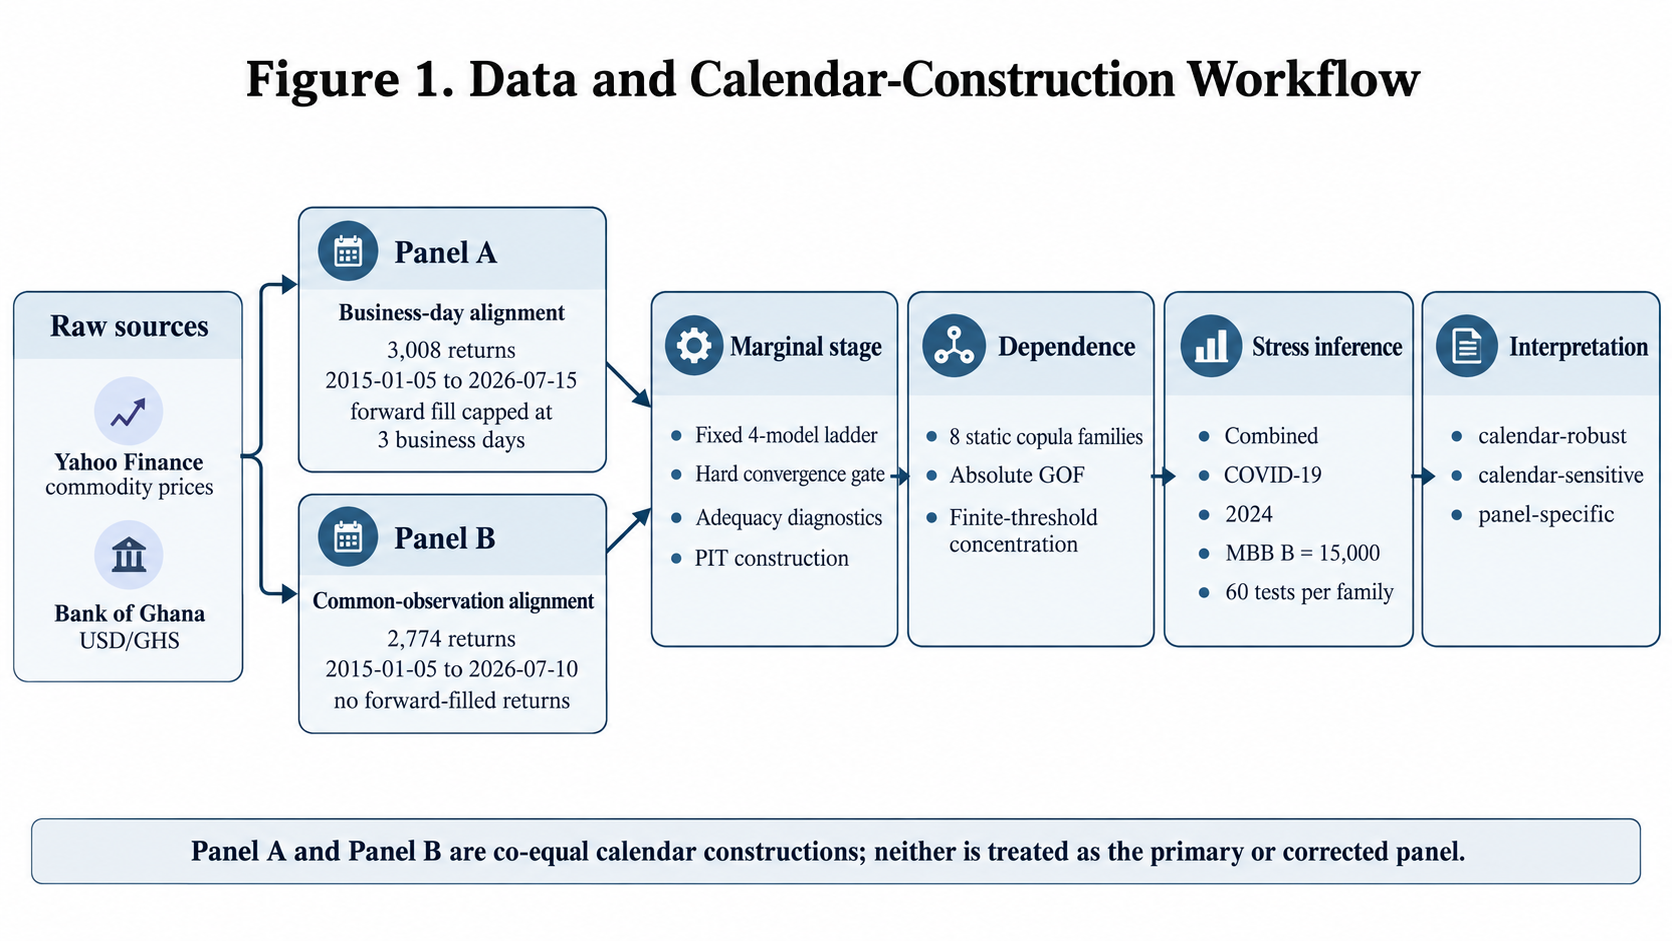
\includegraphics[width=\linewidth]{figures/publication/figure_01_calendar_workflow.png}
\caption{Data and calendar-construction workflow. Panel A uses business-day alignment with forward filling capped at three business days, whereas Panel B uses consecutive common actual-source observation dates without forward-filled returns. The two panels are treated as co-equal representations of the observation process.}
\label{fig:calendar-workflow}
\end{figure}

\subsection{Empirical finite-threshold tail-concentration profiles}
\label{sec:results-tailprofiles}

Figure~\ref{fig:tail-profiles} presents empirical lower- and upper-tail concentration measures at $q=0.025$, $0.05$, and $0.10$ for selected asset pairs under both calendar constructions. These quantities are finite-threshold empirical concentration measures and are not interpreted as asymptotic tail-dependence coefficients.

Across the selected pairs, concentration generally increases as the threshold widens from $q=0.025$ to $q=0.10$, although the magnitude and degree of agreement between Panels A and B vary across asset combinations. Cocoa--Gold displays broadly similar profiles under the two calendar constructions, particularly at the intermediate and wider thresholds. Cocoa--Brent shows clearer separation between the lower and upper tails, with lower-tail concentration exceeding upper-tail concentration throughout most of the threshold range in both panels.

Gold--WTI exhibits comparatively pronounced concentration in both tails, particularly at $q=0.10$. Although some panel-specific differences are present at the more extreme thresholds, both calendar constructions indicate substantial finite-threshold concentration for this pair as the threshold widens. Gold--Cedi, by comparison, displays lower concentration levels overall and somewhat greater differences between the two calendar constructions, particularly in the lower tail at the wider threshold.

The comparison therefore indicates that some empirical tail features are relatively stable to calendar construction whereas others are more sensitive to the treatment of nonsynchronous observations. This distinction motivates the subsequent absolute copula goodness-of-fit analysis rather than treating the empirical profiles alone as evidence of a particular parametric dependence structure.

\begin{figure}[htbp]
\centering
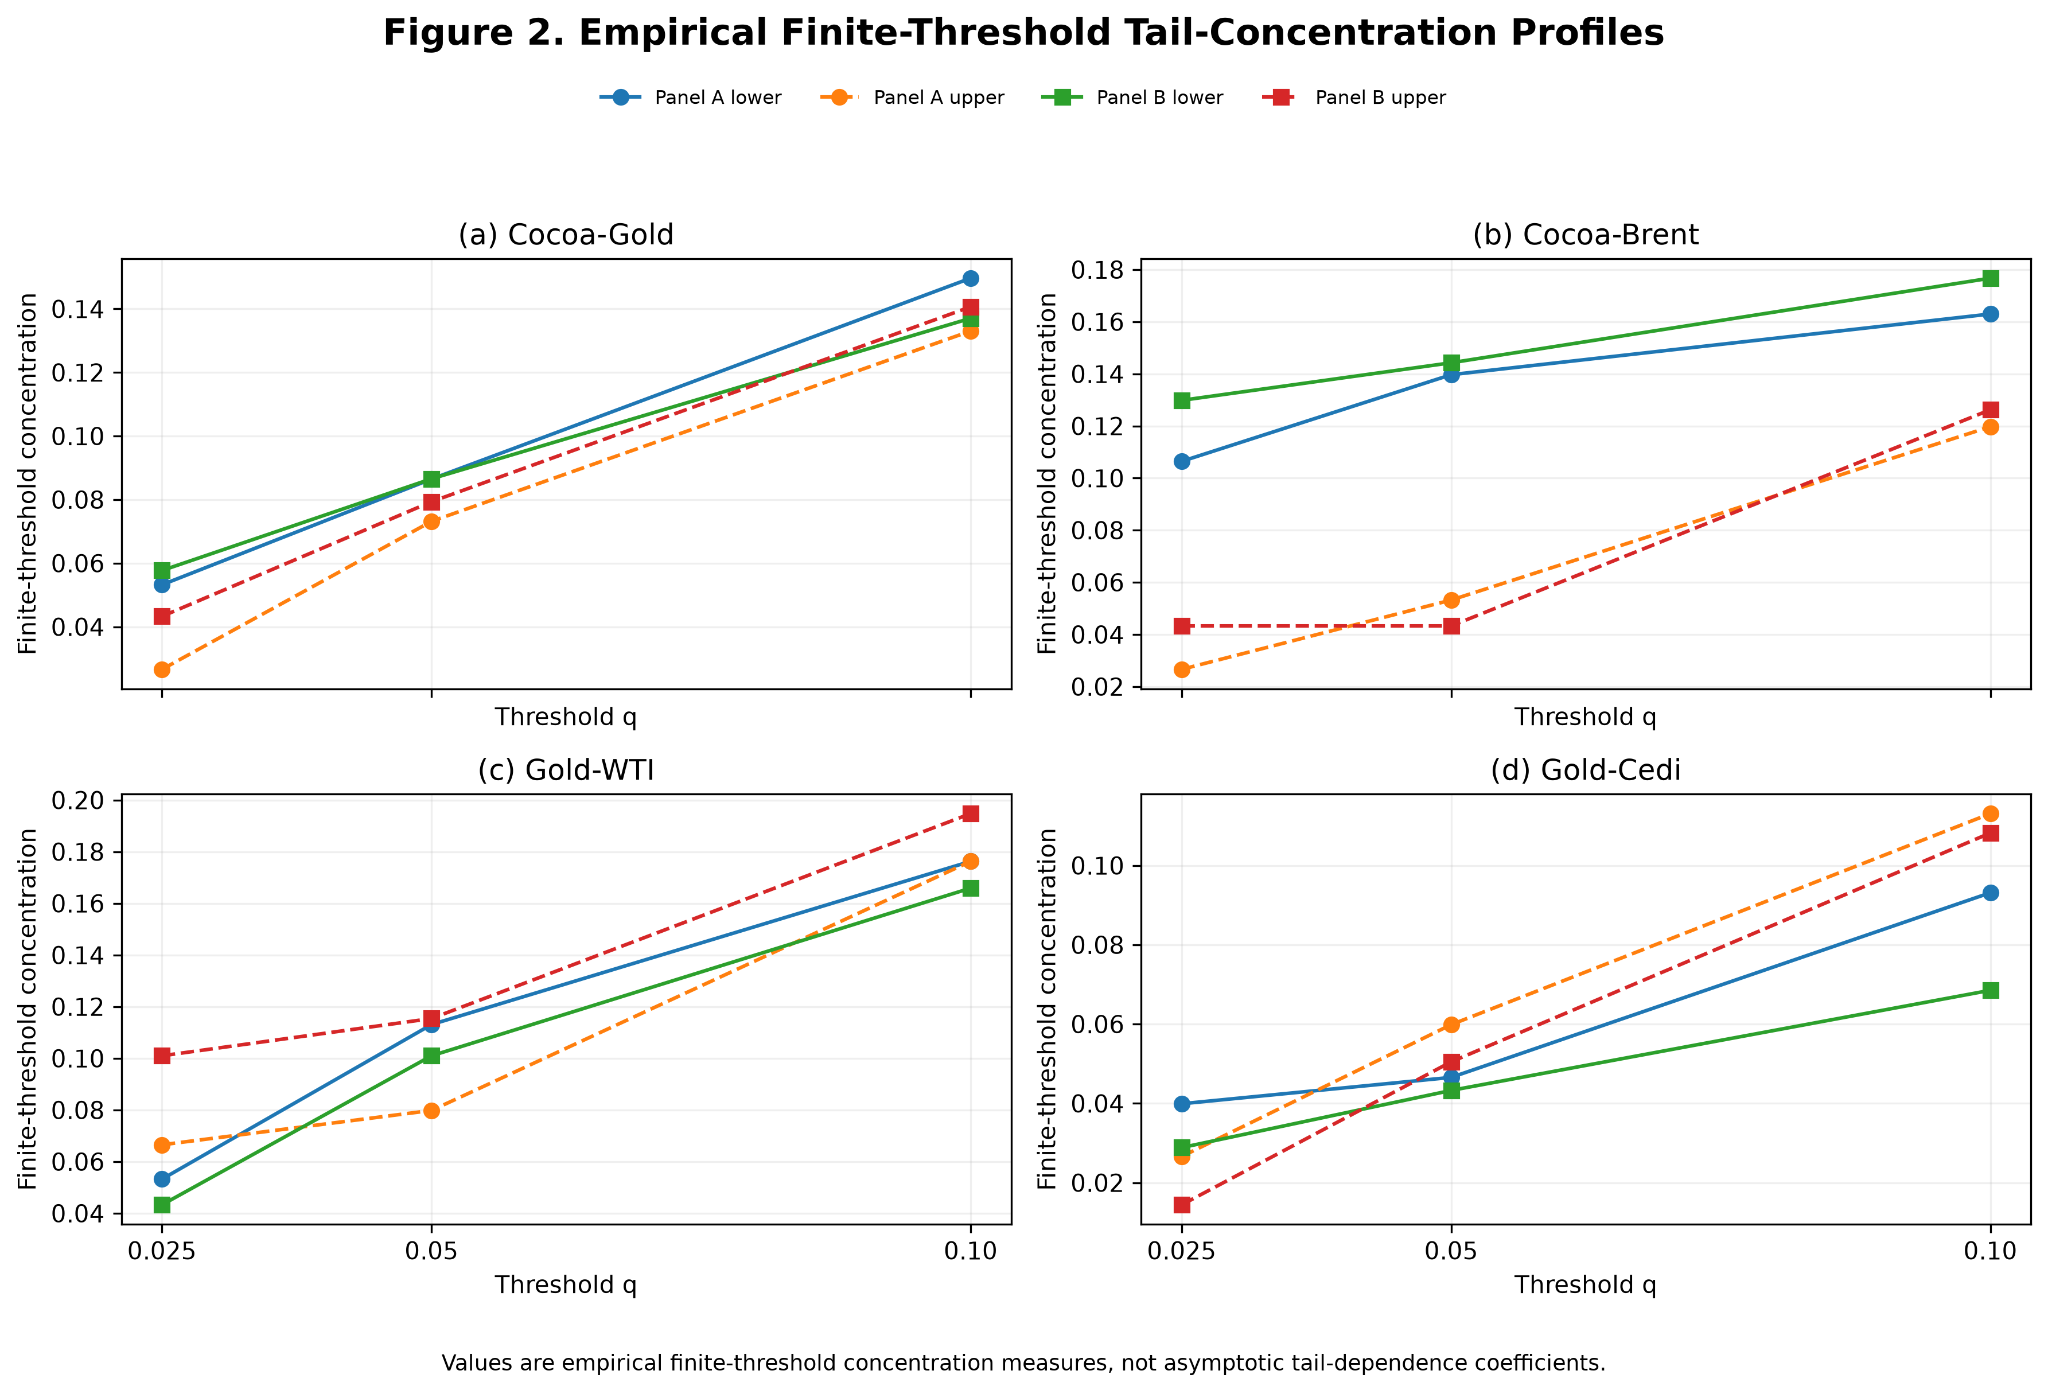
\includegraphics[width=\linewidth]{figures/publication/figure_02_tail_concentration_profiles.png}
\caption{Empirical finite-threshold tail-concentration profiles. Lower- and upper-tail empirical concentration at $q=0.025$, $0.05$, and $0.10$ for selected pairs under Panels A and B. The values are finite-threshold concentration measures and should not be interpreted as asymptotic tail-dependence coefficients.}
\label{fig:tail-profiles}
\end{figure}

\subsection{Static copula goodness-of-fit across calendar constructions}
\label{sec:results-gof}

Substantial differences emerge across asset pairs in the ability of the eight tested static copula families to pass the absolute goodness-of-fit assessment (Figure~\ref{fig:gof-heatmap}). Three commodity--commodity pairs---Gold--Brent, Gold--WTI, and Brent--WTI---produce a calendar-robust pattern of complete rejection. For each of these pairs, all eight tested static copula families are rejected in both Panel A and Panel B. The result therefore does not depend on the choice between the business-day and common-observation calendar constructions.

The four commodity--Cedi pairs show the opposite pattern. For Cocoa--Cedi, Gold--Cedi, Brent--Cedi, and WTI--Cedi, all eight tested families are non-rejected in both calendar constructions. This result is interpreted strictly as an absence of rejection under the applied goodness-of-fit tests; it does not establish that any particular copula family is the true dependence model.

The strongest calendar sensitivity occurs among the three Cocoa--commodity pairs. In Panel A, none of the eight families is non-rejected for Cocoa--Gold, Cocoa--Brent, or Cocoa--WTI, corresponding to complete eight-family rejection. In Panel B, however, six of eight families are non-rejected for Cocoa--Gold, while five of eight are non-rejected for both Cocoa--Brent and Cocoa--WTI. Thus, the absolute goodness-of-fit assessment for the Cocoa--commodity relationships depends materially on the observation-calendar construction.

The results therefore separate the asset pairs into three evidential categories: calendar-robust model inadequacy for Gold--Brent, Gold--WTI, and Brent--WTI; calendar-robust non-rejection for the four commodity--Cedi pairs; and calendar-sensitive adequacy for the three Cocoa--commodity pairs.

\begin{figure}[htbp]
\centering
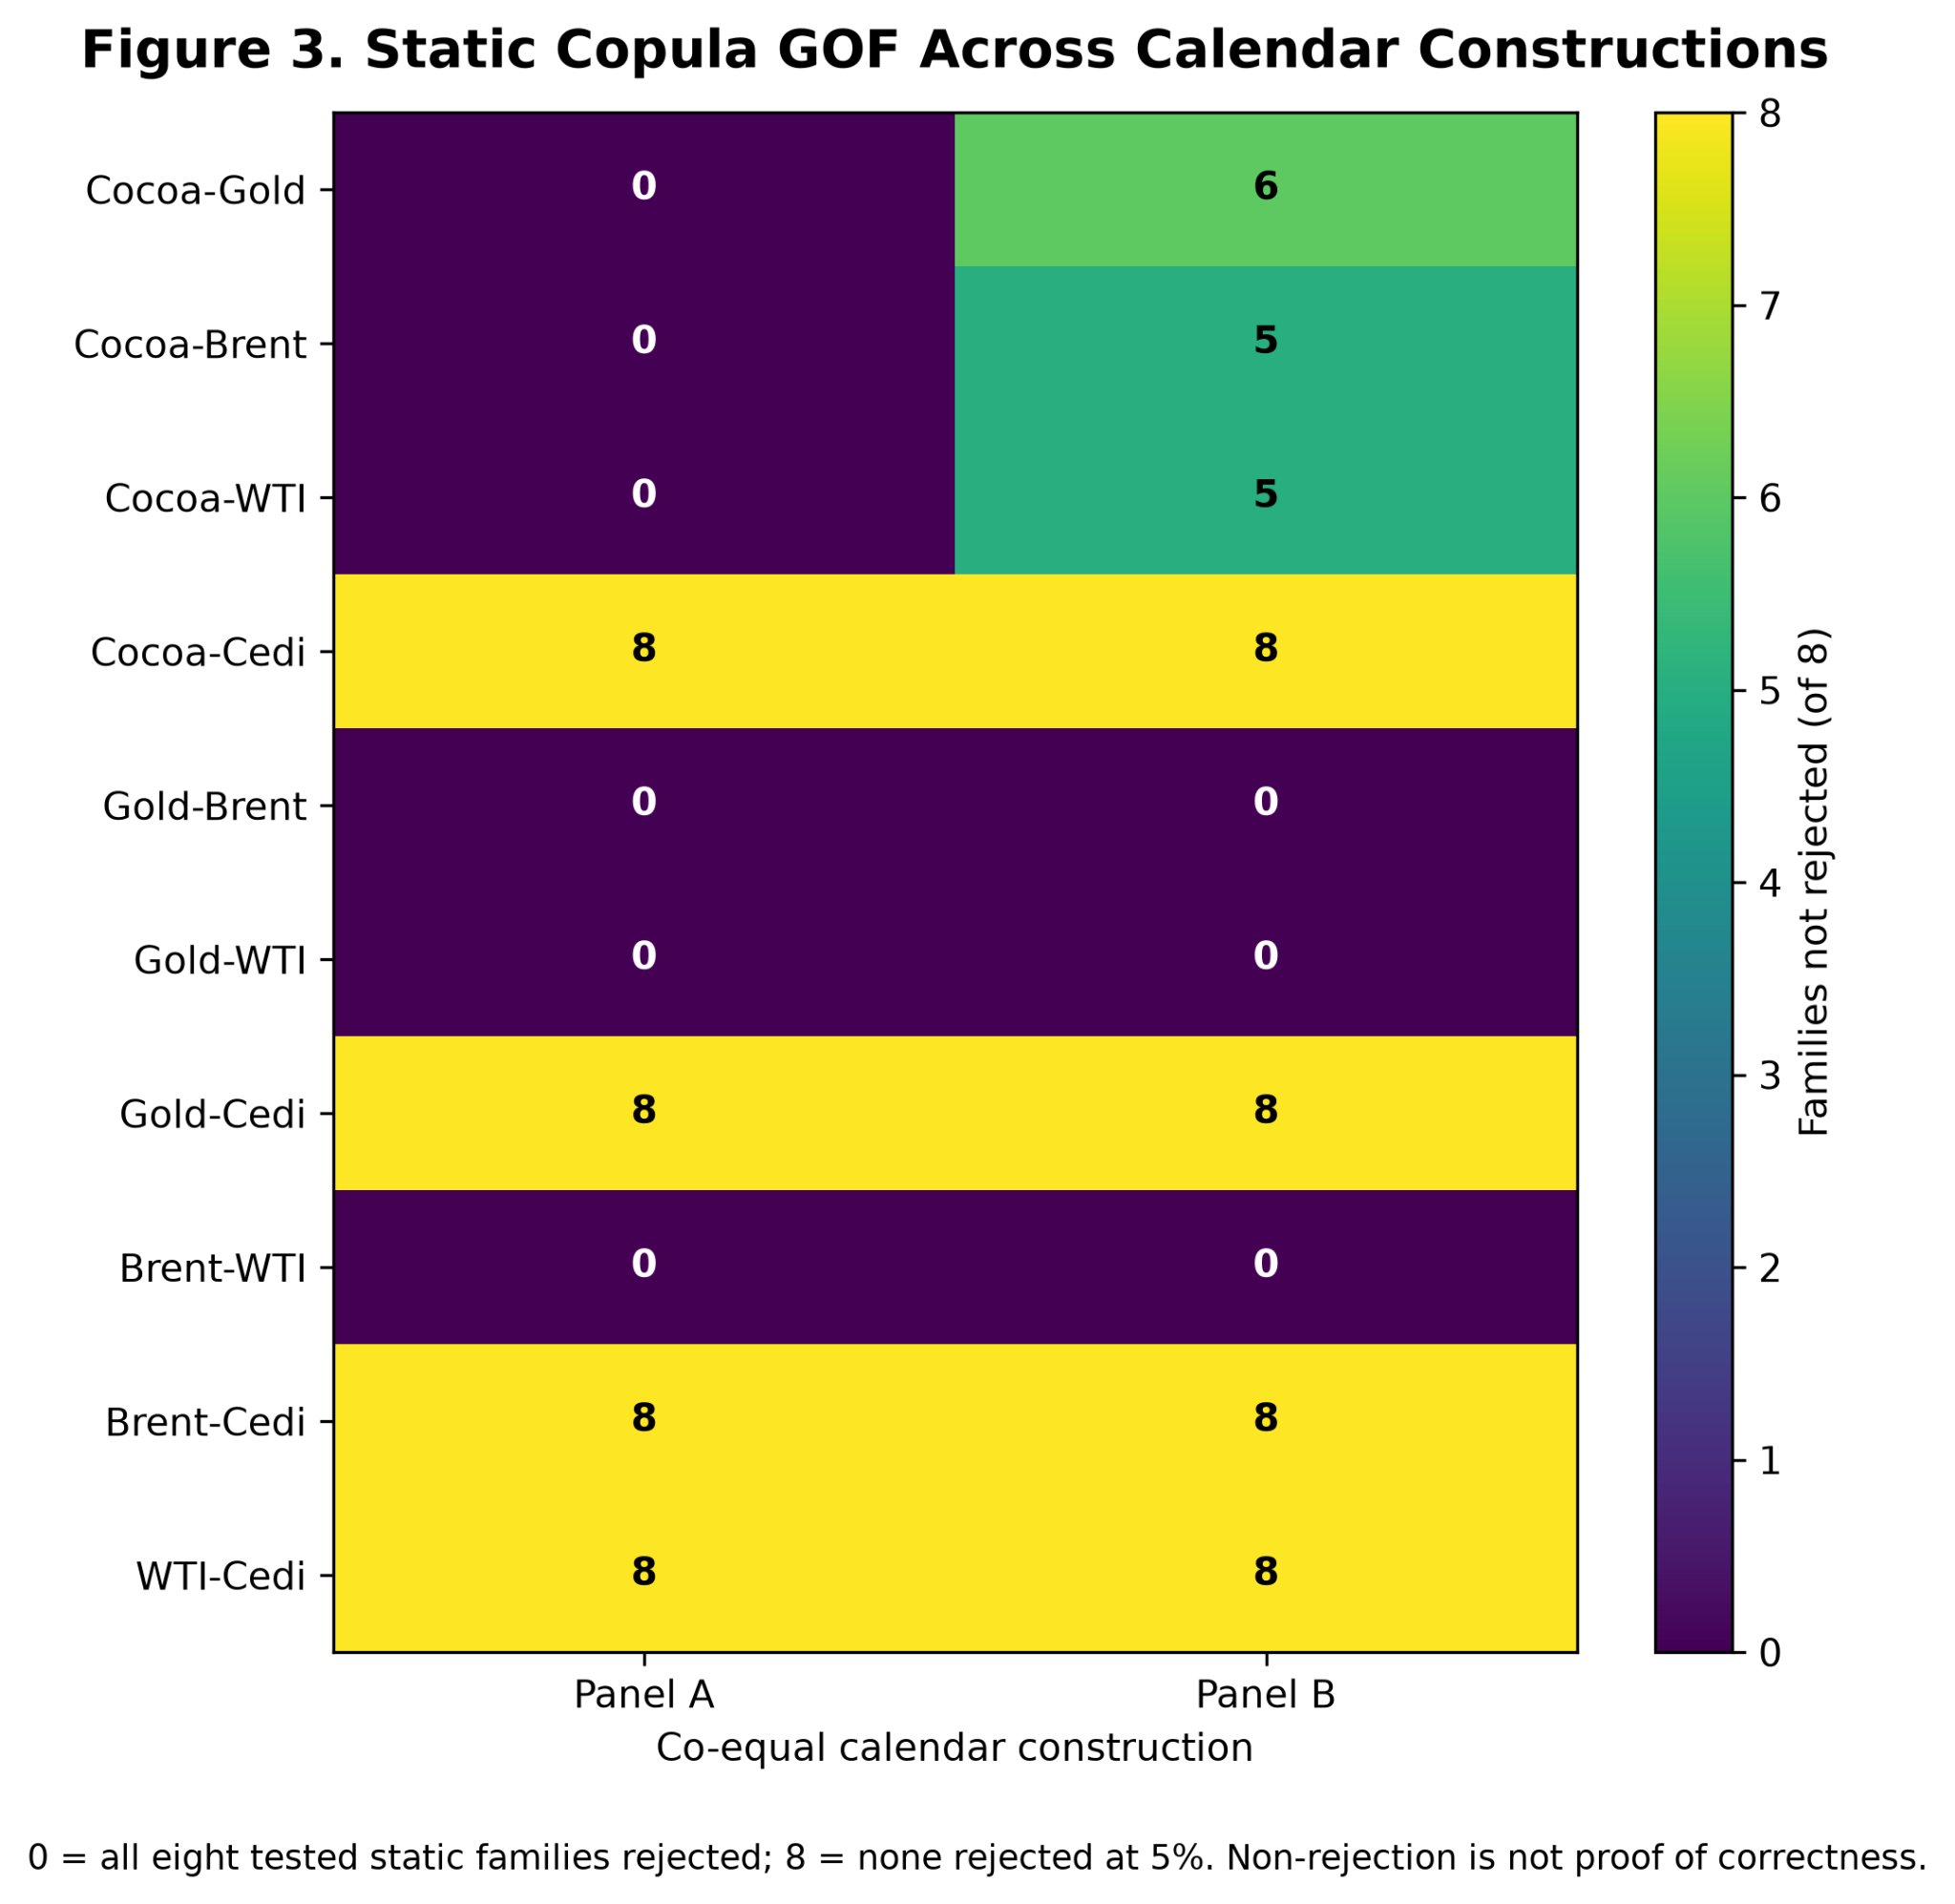
\includegraphics[width=0.82\linewidth]{figures/publication/figure_03_copula_gof_heatmap.png}
\caption{Static copula goodness-of-fit across calendar constructions. Each cell reports the number of the eight tested static copula families that were not rejected at the 5\% level. A value of zero indicates rejection of all eight tested families, whereas eight indicates that none was rejected. Non-rejection should not be interpreted as proof of model correctness.}
\label{fig:gof-heatmap}
\end{figure}

\subsection{Stress--calm tail-concentration inference}
\label{sec:results-calmstress}

Stress--calm comparisons were conducted separately for the combined stress definition, the COVID-19 period, and the 2024 stress period, with 60 tests undertaken within each panel--stress family. Figure~\ref{fig:stress-summary} distinguishes the nominal $p<0.05$ counts from the multiplicity-controlled results.

For the combined stress definition, 6 of 60 tests are nominally significant in Panel A and 5 of 60 in Panel B. The COVID-19 specification produces the largest number of nominal findings, with 13 of 60 tests in Panel A and 11 of 60 in Panel B. Under the 2024 specification, 6 of 60 tests are nominally significant in Panel A and 7 of 60 in Panel B.

These unadjusted counts do not translate into multiplicity-controlled discoveries. Across all three stress definitions and both calendar constructions, zero tests survive Bonferroni correction and zero survive Benjamini--Hochberg false-discovery-rate correction. Accordingly, the nominal $p<0.05$ findings are retained only as descriptive diagnostics and are not promoted to confirmatory evidence of stress-related changes in tail concentration.

The consistency of the adjusted result across the two calendar constructions is particularly important. Although the number and identity of nominal findings vary to some extent between Panels A and B, the inferential conclusion after multiplicity control is invariant: the analysis does not identify a stress--calm tail-concentration difference that meets the prespecified multiplicity-controlled evidential threshold.

\begin{figure}[htbp]
\centering
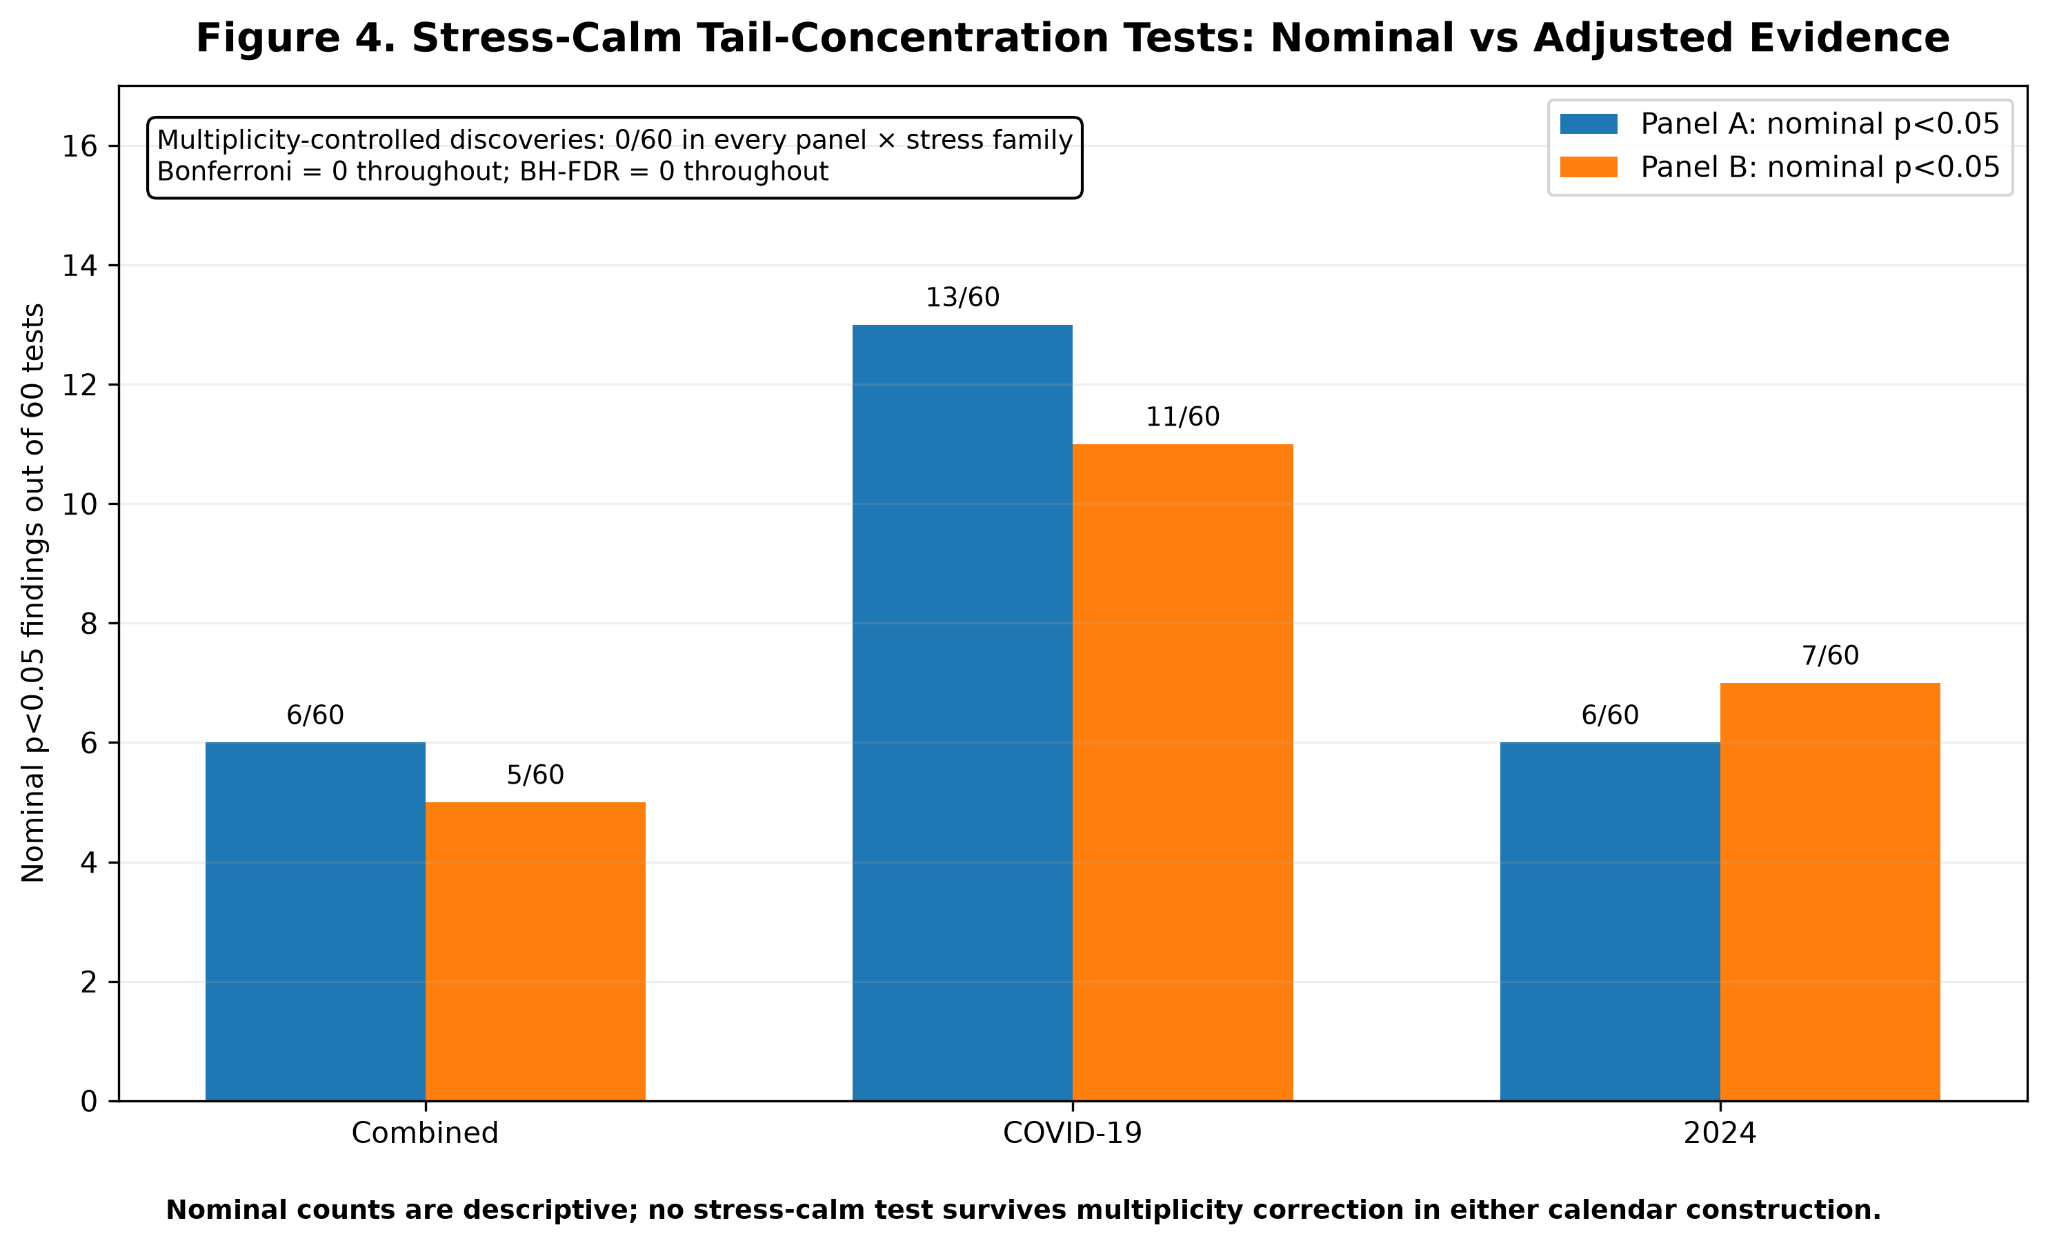
\includegraphics[width=\linewidth]{figures/publication/figure_04_stress_summary.png}
\caption{Stress--calm tail-concentration tests: nominal versus adjusted evidence. Bars show the number of nominal $p<0.05$ findings among 60 tests for each stress definition. None of the tests survives either Bonferroni or Benjamini--Hochberg correction in either calendar construction.}
\label{fig:stress-summary}
\end{figure}

\subsection{Cedi-related diagnostics and sensitivity analyses}
\label{sec:results-cedi}

Additional analyses were undertaken because the selected Cedi marginal reference model did not satisfy the marginal adequacy requirement in either calendar construction. The Cedi-related dependence and extreme-value results are therefore interpreted conditionally on this limitation rather than being treated as unrestricted model-based evidence.

The Panel B peaks-over-threshold analysis shows sensitivity in the estimated generalized Pareto shape parameter, 99\% Value-at-Risk, and 99\% Expected Shortfall as the threshold quantile varies (Supplementary Figure~\ref{fig:s1-evt}). The $q=0.90$ specification is retained as a reference point in the sensitivity display, but the resulting EVT quantities remain conditional diagnostics because of the unresolved Cedi marginal inadequacy.

The Panel A A--G sensitivity exercise likewise demonstrates that nominal findings vary with the treatment applied to the Cedi series (Supplementary Figure~\ref{fig:s2-ag}). The number of nominal $p<0.05$ findings across the seven treatments is 3, 3, 2, 0, 2, 2, and 2, respectively. In particular, treatment D produces no nominal findings. For the illustrated Brent--Cedi lower-tail comparison at $q=0.05$, several alternative treatments yield unadjusted $p$-values below 0.05, whereas treatment D yields $p=0.641$. These results reinforce the sensitivity of unadjusted Cedi-related findings to data treatment and support their classification as diagnostics rather than headline discoveries.

The separate PIT-clipping audit provides evidence that the observed numerical clipping artifact is negligible for the prespecified tail analysis (Supplementary Figure~\ref{fig:s3-pit}). Three Cedi observations are tied at the clipping boundary of $10^{-6}$. Recovering their residual ordering alters only two pseudo-observations, does not change membership of the $q=0.025$, $0.05$, or $0.10$ tail sets, and produces a maximum absolute change in the observed goodness-of-fit statistic of approximately $0.000262$. Thus, although the clipping artifact is explicitly investigated, it does not account for the substantive cross-panel results reported above.

\subsection{Cross-panel synthesis of the evidence}
\label{sec:results-synthesis}

Table~\ref{tab:crosspanel} summarizes the findings that are robust and those that are sensitive to calendar construction. Several results are stable across both panels. All four commodity--Cedi pairs have all eight tested static copula families non-rejected under both calendar constructions. Conversely, Gold--Brent, Gold--WTI, and Brent--WTI show complete eight-family rejection in both panels. Most importantly for the stress analysis, neither panel produces any Bonferroni- or BH-FDR-adjusted stress--calm discovery under the combined, COVID-19, or 2024 stress definitions.

The principal calendar-sensitive findings concern Cocoa's dependence with the other commodities. Cocoa--Gold, Cocoa--Brent, and Cocoa--WTI produce complete rejection of all eight static copula families under Panel A, whereas Panel B retains six, five, and five non-rejected families, respectively. These results show that the inferred adequacy of conventional static copulas for the Cocoa--commodity relationships is sensitive to the treatment of nonsynchronous trading calendars.

Taken together, the results support three evidential classifications used throughout the remainder of the study: \emph{calendar-robust findings}, for which the substantive result is preserved under both calendar constructions; \emph{calendar-sensitive findings}, for which the inference changes with the observation-calendar treatment; and \emph{panel-specific diagnostics}, which are informative within one construction but are not promoted to cross-panel conclusions.

The strongest cross-panel conclusions are therefore not based on the number of nominal findings alone, but on the combination of absolute model adequacy, robustness to calendar construction, and multiplicity-controlled inference.

\begin{table}[htbp]
\centering
\caption{Cross-panel evidence summary.}
\label{tab:crosspanel}
\small
\begin{tabular}{p{0.22\linewidth}p{0.34\linewidth}p{0.34\linewidth}}
\toprule
Feature & Panel A: business-day alignment & Panel B: common-observation alignment \\
\midrule
Return observations & 3,008 & 2,774 \\
Return period & 2015-01-05 to 2026-07-15 & 2015-01-05 to 2026-07-10 \\
Alignment rule & Business-day; forward fill $\leq 3$ business days & Consecutive common actual-source dates \\
Commodity--Cedi GOF & All 4 pairs: 8/8 not rejected & All 4 pairs: 8/8 not rejected \\
Robust 0/8 not rejected & Gold--Brent; Gold--WTI; Brent--WTI & Gold--Brent; Gold--WTI; Brent--WTI \\
Cocoa commodity pairs & 0/8 not rejected for all 3 pairs & 6/8, 5/8, 5/8 not rejected \\
Corrected stress discoveries & 0 under all 3 families & 0 under all 3 families \\
Role & Co-equal panel & Co-equal panel \\
\bottomrule
\end{tabular}
\end{table}

% Supplementary diagnostic figures. These can be moved to a separate
% supplement file when the target journal's submission format is fixed.
\begin{figure}[htbp]
\centering
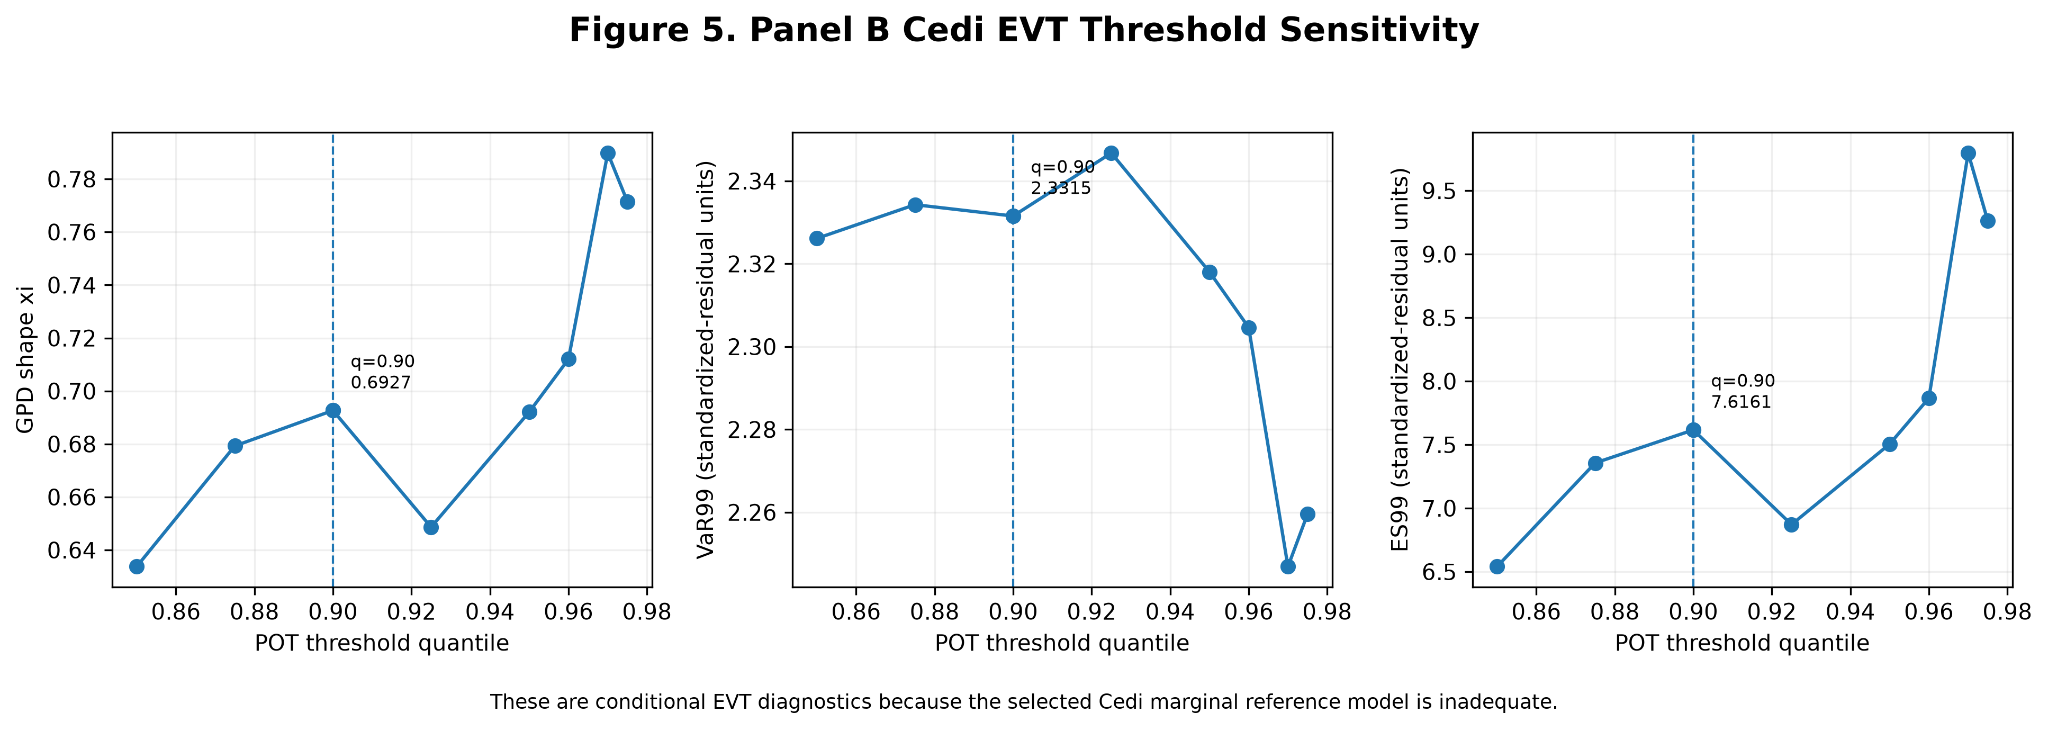
\includegraphics[width=\linewidth]{figures/publication/figure_S1_cedi_evt_threshold_sensitivity.png}
\caption{Panel B Cedi EVT threshold sensitivity. These are conditional diagnostics because the selected Cedi marginal reference model is inadequate.}
\label{fig:s1-evt}
\end{figure}

\begin{figure}[htbp]
\centering
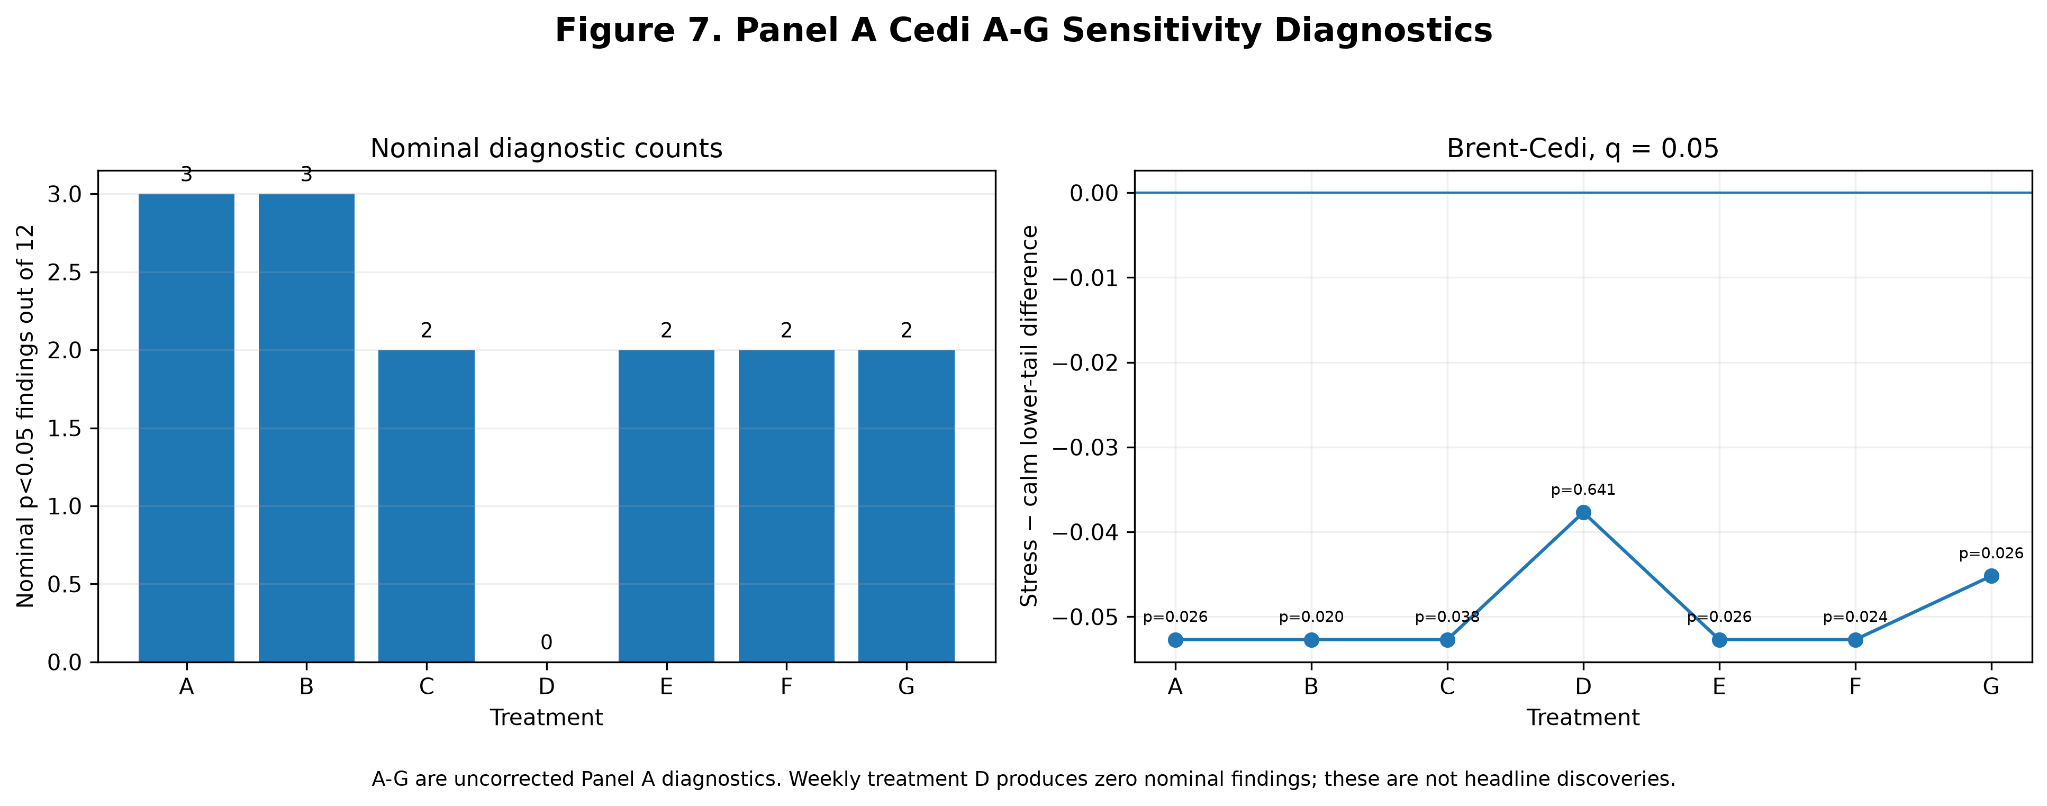
\includegraphics[width=\linewidth]{figures/publication/figure_S2_cedi_AG_sensitivity.png}
\caption{Panel A Cedi A--G sensitivity diagnostics. The displayed counts and $p$-values are uncorrected diagnostics and are not treated as headline discoveries.}
\label{fig:s2-ag}
\end{figure}

\begin{figure}[htbp]
\centering
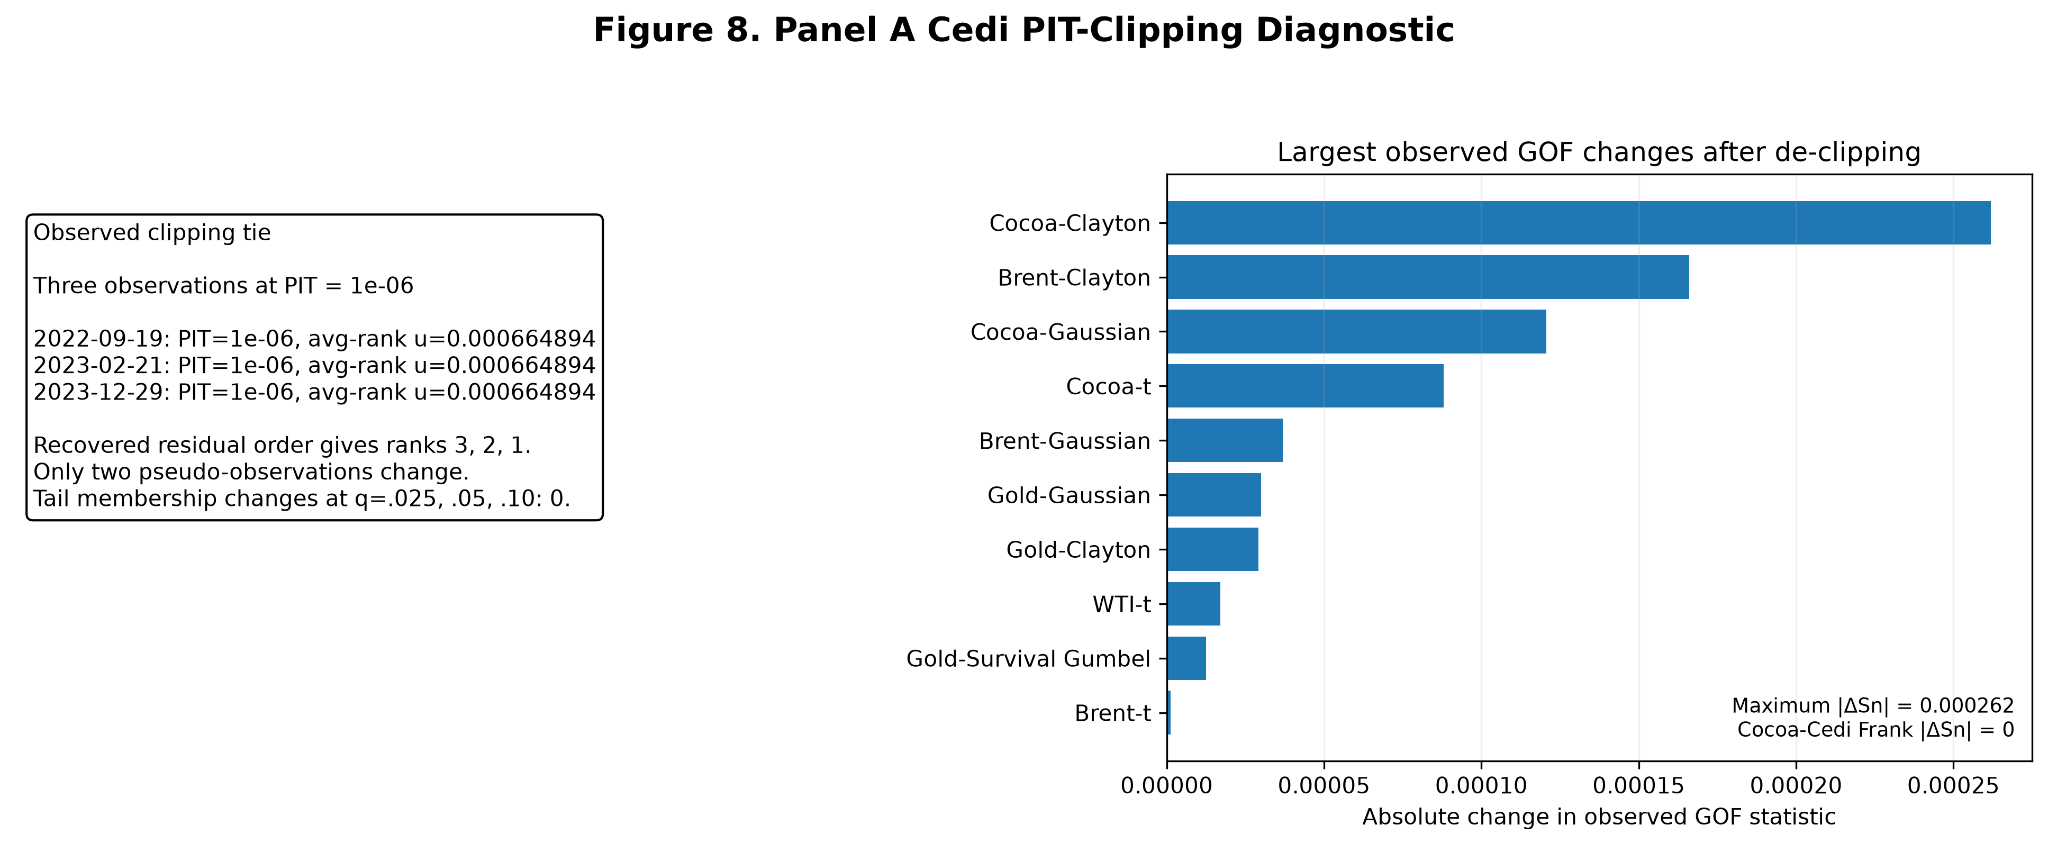
\includegraphics[width=\linewidth]{figures/publication/figure_S3_pit_clipping_diagnostic.png}
\caption{Panel A Cedi PIT-clipping diagnostic. The observed clipping tie has negligible numerical consequences for the prespecified tail sets and copula goodness-of-fit statistics.}
\label{fig:s3-pit}
\end{figure}


\section{Robustness}
\label{sec:robustness}

We summarize four robustness checks here; full detail is in
Appendices~\ref{app:pinksheet}--\ref{app:cedi-robustness}.

\textbf{Roll effects.} Comparing Yahoo futures returns, resampled to
match the World Bank Pink Sheet's monthly-average methodology, against
the Pink Sheet's independent non-futures benchmark gives return
correlations of 0.98 (Brent), 0.99 (WTI), 0.94 (cocoa) and 0.997 (gold)
-- all high enough to rule out roll contamination as a material concern
for the daily analysis. An initial, methodologically mismatched
comparison (Yahoo month-end snapshots against Pink Sheet monthly
averages) gave correlations as low as 0.62; the gap between that number
and the properly matched 0.94 illustrates how much of an apparent
data-quality problem can be a sampling-convention artifact rather than a
genuine one, a distinction worth verifying explicitly rather than
assuming.

\textbf{Weekly frequency.} Resampling to weekly closes and re-estimating
the full pipeline reproduces the same qualitative pattern as daily data:
no pair shows a significant tail-dependence increase during stress at
either the uncorrected or corrected level.

\textbf{Cedi marginal treatment.} Across six independent treatments of
the cedi's difficult marginal -- the baseline GARCH filter, unfiltered
raw ranks, an ARMA-only filter, weekly frequency, an explicit hurdle
model, and a two-state Markov-switching extension -- the four cedi-pair
findings are stable with one instructive exception: Gold--Cedi's
apparent significance under the baseline treatment ($p=0.036$)
disappears under every more careful alternative ($p=0.08$--$0.15$),
indicating that specific result was an artifact of the baseline
marginal specification rather than a robust feature of the data.
Cocoa--Cedi is never close to significant under any treatment;
WTI--Cedi is consistently significant uncorrected but is the pair
already resolved by the correction and disaggregation results above;
Brent--Cedi is a genuine borderline case across every treatment,
strengthening modestly under the most sophisticated (Markov-switching)
specification -- reported honestly as an open, unresolved sensitivity
rather than smoothed over in either direction.

\textbf{Marginal specification versus model risk.} Neither the hurdle
model nor the Markov-switching extension achieves full distributional
adequacy by the Kolmogorov--Smirnov standard, despite each representing
a genuine improvement in how the cedi's zero-inflated, regime-dependent
structure is modelled (Appendix~\ref{app:cedi-robustness} reports a
roughly forty-fold improvement in Bayesian Information Criterion between
a single Gaussian and a two-regime mixture, for instance). We read this
as a second, independent instance of this paper's central model-risk
finding: the cedi's marginal difficulty is not merely a matter of
insufficiently flexible tools -- it persists across six increasingly
sophisticated attempts -- in exactly the same way that the
commodity-commodity copula rejection persists across eight increasingly
varied candidate families.

\section{Discussion: implications for risk management}
\label{sec:discussion}

We frame our results around the two risks distinguished in the
introduction, since conflating them would understate the paper's
findings on one dimension and overstate them on the other.

\textbf{On economic exposure.} Ghana's commodity exposure should not be
assumed to intensify automatically during a crisis. Across ninety tests
spanning three stress-window definitions, we find no dependence increase
that survives correction for multiple testing. This has a direct,
actionable implication for reserve and buffer management: sizing
commodity stress buffers on the assumption of crisis-amplified joint
risk, when the data do not support that assumption, would misallocate
scarce reserves toward a risk that is not detectably present, at the
expense of risks that are. The one clear exception -- the strong,
stable Brent--WTI linkage -- has a correspondingly direct implication:
oil-price exposure should be sized as a single joint risk, not treated
as internally diversified across the two benchmarks.

\textbf{On model risk.} This is where we believe the paper's more
novel contribution lies. That six of ten pairs reject every one of eight
standard copula families is not an abstract methodological footnote; it
means that any risk model built on these families for these pairs is,
by construction, fitting the wrong shape to real, substantial,
precisely-measured dependence. A risk manager relying on a Gaussian or
even a Student-$t$ copula for cocoa-oil or cocoa-gold exposure is not
missing a small amount of tail risk -- they are using a model the data
itself rejects at conventional significance, for a dependence structure
that is real and sizeable. The same logic applies to the cedi's own
marginal distribution, which resists adequate description under
GARCH filtering, an explicit zero-inflated hurdle specification, and a
Markov-switching regime model alike. For institutions building
commodity or currency risk models on similarly difficult emerging-market
series, the appropriate response is not to pick a convenient family and
proceed, but to test goodness-of-fit explicitly and disclose when no
standard family passes, exactly as we do here.

\textbf{On the cedi's own risk profile.} Independently of any commodity
link, the cedi's extreme-value shape parameter ($\hat\xi = 0.67$) is
roughly four times the heaviest commodity tail in this panel. This is a
more clearly evidenced risk than any commodity-transmission channel we
test, and argues for monitoring cedi depreciation risk on its own
extreme-value terms -- reserve buffers and hedging calibrated to the
currency's own tail behaviour -- rather than treating it as a derivative
quantity of commodity shocks that this paper does not find robust
evidence for at daily-to-monthly frequency.

\textbf{On monitoring system design.} A practical lesson from
Section~\ref{sec:results-calmstress}'s methodological note is directly
transferable to any institution building a similar tail-risk monitor:
a single nominally significant result, even one surviving a
formal multiple-testing correction, is not sufficient evidence of a real
effect until checked against (a) an independent, higher-resolution
re-estimation to rule out coarse-bootstrap artifacts, and (b) a natural
alternative definition of the event window being tested. Both checks
changed our own conclusions during this analysis; a monitoring system
that skipped either would have reported false signals with a
misleadingly precise-looking $p$-value attached.

\section{Limitations}
\label{sec:limitations}

\textbf{Marginal inadequacy for two of five series.} Brent and the cedi
fail every specification tried and are retained at best-AIC. For the
cedi, six independent treatments -- described in full in
Section~\ref{sec:robustness} -- establish that our tail-dependence
conclusions do not depend on this choice, but any single point estimate
involving Brent or the cedi inherits some uncertainty from unresolved
marginal misspecification.

\textbf{Limited independent stress episodes.} Our entire inferential
apparatus rests on two episodes. Section~\ref{sec:results-calmstress}
demonstrates directly that this is enough to generate an apparently
significant result under one reasonable stress-window definition that a
higher-resolution bootstrap and an alternative window definition both
resolve as non-robust. A longer sample incorporating additional
independent episodes -- Ghana's 2014--2015 currency crisis, not included
here since daily commodity futures data was fetched only from 2015
onward -- would materially strengthen this test's power.

\textbf{Copula family coverage.} Even at eight candidate families, six
pairs reject every one. Vine copulas or a fully nonparametric copula
surface estimate are natural next steps our framework does not attempt.

\textbf{Bonferroni scope.} Our family-wise correction spans all sixty
cells within each stress-window definition; it does not additionally
correct across the three stress-window definitions tested (combined,
COVID-only, 2024-only), a further, more conservative layer we did not
apply.

\textbf{Transmission analysis power.} The monthly regressions run on
88--127 observations, short by the standards of time-series
econometrics, and should be read as a modest first-pass extension.

\section{Conclusion}
\label{sec:conclusion}

We provide a copula--extreme-value-theory framework for measuring
extreme co-movement among Ghana's three dominant export commodities and
its transmission to the official exchange rate, built on the Bank of
Ghana's own reference series rather than a free-data proxy of documented
poor quality. Applied to real data from 2015 to 2026, the framework does
not find robust evidence of stress-driven tail-dependence intensification
among cocoa, gold and crude oil -- a conclusion holding across three
distinct stress-window definitions, two independent multiple-testing
corrections, and a dedicated re-verification of the one result that
initially appeared to survive correction. Independently, the same
framework identifies a concrete, quantified model-risk problem: standard
copula families, even substantially expanded beyond the conventional
four, cannot adequately describe real commodity-commodity dependence for
six of ten tested pairs, and the cedi's own difficult marginal resists
six increasingly sophisticated modelling attempts. For a commodity-
dependent economy's risk-management practice, we read this as two
separable messages that should not be collapsed into one: Ghana's
export-commodity exposure should not be assumed to compound
automatically in every crisis, but the tools used to measure that
exposure carry model risk substantial enough to deserve equal weight in
any risk-management framework built on them.

\section*{Data availability statement}
The complete analysis pipeline, all output tables underlying every
figure and table in this paper, and a machine-readable verification
ledger recording the source of every quantitative claim are available at
\url{https://github.com/Jonathanerrils/tail-dependence-ghana}. Raw
commodity futures prices are not redistributed, per Yahoo Finance's
terms of service; the fetch script that reproduces them locally is
provided instead. Bank of Ghana source tables are redistributed with
attribution.

\section*{Code availability statement}
All analysis code (Python 3.12; \texttt{arch}, \texttt{statsmodels},
\texttt{scikit-learn}, \texttt{hmmlearn}, \texttt{scipy}) is available at
the repository above under an open-source license, including the scripts
used to produce every table and figure in this paper.

\section*{Funding statement}
This research received no external funding.

\section*{Conflict of interest statement}
The author declares no conflict of interest.

\section*{Author contributions statement}
Conceptualization, methodology, software, formal analysis, data
curation, writing, and verification: J.N.

\section*{Note on the use of AI assistance}
Portions of the code implementation, data verification, and manuscript
drafting for this paper were carried out with the assistance of an AI
language model (Anthropic's Claude), used as a research and writing
tool under the author's direction, review, and verification throughout.
All modelling decisions, empirical results, and their interpretation
are the author's responsibility.

\section*{Note on bibliography style}
This paper uses the Harvard (author--year) elsarticle bibliography
style (\texttt{elsarticle-harv.bst}) throughout, for readability in a
literature-heavy introduction and discussion, and as standard practice
in this paper's target journal set.

\bibliographystyle{elsarticle-harv}
\bibliography{references}

\section*{Figures}

\begin{figure}[htbp]
\centering

\includegraphics[width=0.95\linewidth]{figures/fig0_prices.png}
\caption{Price levels (index, start = 100), 2015--2026.}
\label{fig:prices}
\end{figure}

\begin{figure}[htbp]
\centering
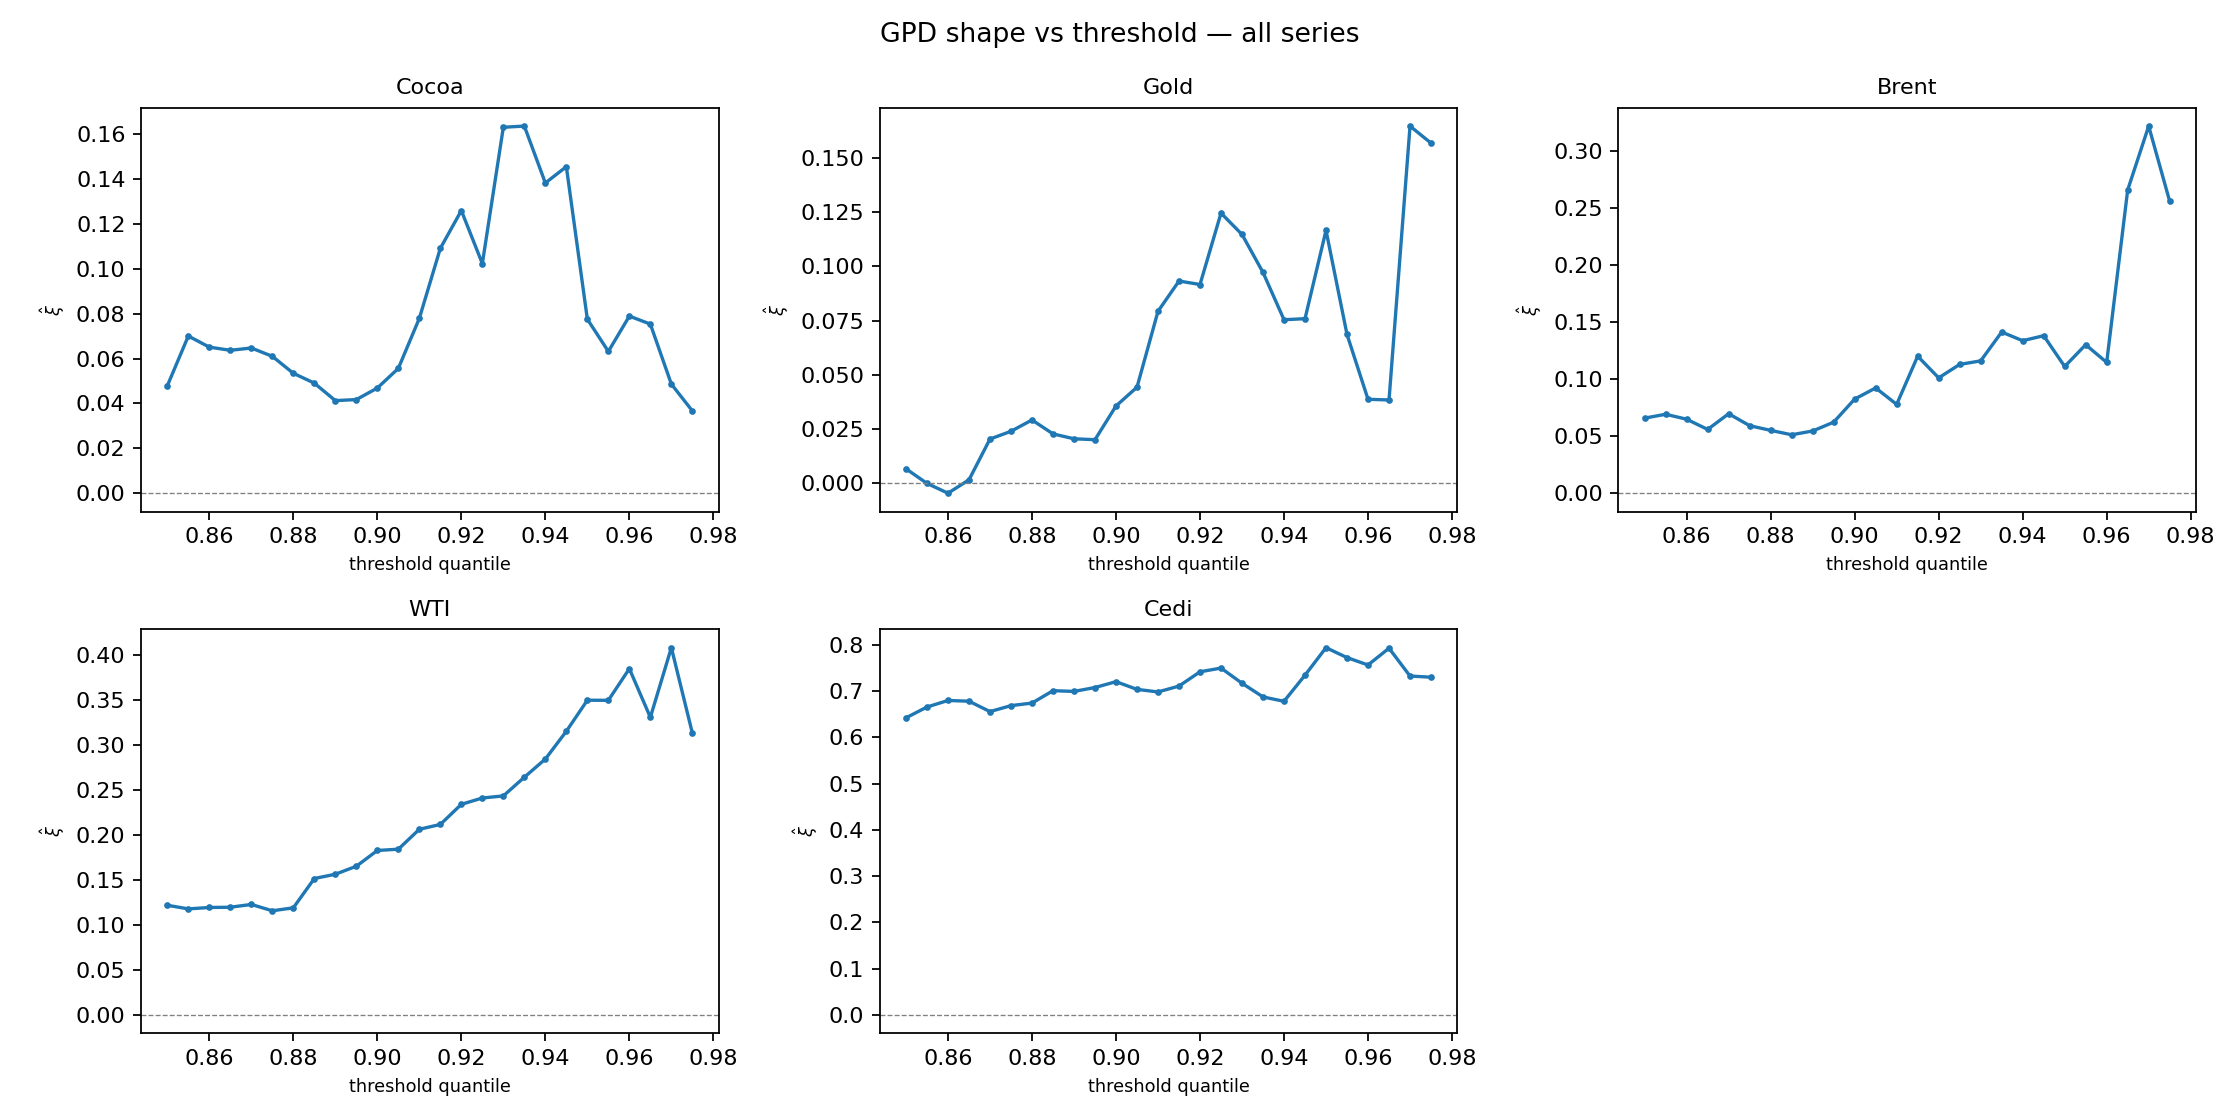
\includegraphics[width=0.85\linewidth]{figures/fig6_threshold_all_series.png}
\caption{GPD shape estimate vs.\ threshold quantile, all five series.}
\label{fig:threshold-all}
\end{figure}

\begin{figure}[htbp]
\centering

\includegraphics[width=0.95\linewidth]{figures/fig5_tail_networks.png}
\caption{Lower-tail dependence networks: calm periods (left) vs.\ 2024 cocoa-shock window (right). Edge weight is empirical $\hat\lambda_L$ ($q=0.05$).}
\label{fig:networks}
\end{figure}

\begin{figure}[htbp]
\centering

\includegraphics[width=0.95\linewidth]{figures/fig4_rolling_tail_dependence.png}
\caption{Rolling 250-day nonparametric empirical $\hat\lambda_L(q=0.10)$, all ten pairs.}
\label{fig:rolling-empirical}
\end{figure}

\appendix

\section{Roll-effect validation: full detail}
\label{app:pinksheet}

Table~\ref{tab:pinksheet-full} reports both the properly matched
(monthly-mean) and the sampling-mismatched (month-end snapshot)
comparisons in full, for all four futures series against the World Bank
Pink Sheet.

\begin{table}[htbp]
\centering
\caption{Pink Sheet vs.\ Yahoo futures monthly return correlation, both resampling conventions, 137 months.}
\label{tab:pinksheet-full}
\begin{tabular}{lrr}
\toprule
Series & Correlation (mean-matched) & Correlation (snapshot, mismatched) \\
\midrule
Brent & 0.980 & 0.759 \\
WTI   & 0.990 & 0.747 \\
Cocoa & 0.942 & 0.618 \\
Gold  & 0.997 & 0.701 \\
\bottomrule
\end{tabular}
\end{table}

Cocoa's largest single-month discrepancy under the matched comparison
falls in October 2024, inside the cocoa-shock window this paper studies
most closely; WTI's largest discrepancy falls in May 2020, immediately
after the April 2020 negative-settlement event already discussed in
Section~\ref{sec:data}. Both are consistent with genuine extreme
volatility in the underlying market during unusual months, not with a
systematic roll-effect bias.

\section{Full quantile-sensitivity and correction tables}
\label{app:fullcorrection}

The complete sixty-cell table (ten pairs $\times$ three quantiles
$\times$ two tails), with uncorrected, Bonferroni ($m=60$) and
Benjamini--Hochberg significance flags for the combined-stress
definition, and the corresponding tables for the COVID-only and
2024-only disaggregated definitions, are distributed as
\texttt{calm\_stress\_full60\_correction.csv} and
\texttt{calm\_stress\_disaggregated\_FINAL.csv} in the data repository
referenced in the Data Availability Statement, rather than reproduced
in full here.

\section{Full eight-family copula fit and goodness-of-fit tables}
\label{app:fullcopula}

The complete $10 \times 8 = 80$-row fit table (AIC, log-likelihood,
fitted parameters and analytic tail-dependence coefficients for every
family and pair) and the corresponding $80$-row goodness-of-fit table
(Cram\'er--von Mises statistic and bootstrap $p$-value for every family
and pair) are distributed as \texttt{copula\_fits\_8family.csv} and
\texttt{copula\_gof\_8family.csv} in the data repository.

\section{Cedi marginal robustness: full construction detail}
\label{app:cedi-robustness}

\subsection{Hurdle model}

The zero-probability component is a logistic autoregression on the
zero-return indicator, $\mathrm{logit}(p_t) = \beta_0 + \beta_1
I_{t-1} + \beta_2 I_{t-2}$, selected over an AR(1) alternative by AIC.
A likelihood-ratio test against a constant-probability null decisively
rejects the constant-probability specification (statistic 24.0,
$p = 6.1\times 10^{-6}$): zero-return days cluster in time rather than
occurring independently, consistent with the Bank of Ghana holding a
rate fixed for stretches rather than making independent daily decisions.
The continuous component is fit to nonzero returns only, and the
resulting distribution is combined with the zero-probability component
into a single mixture PIT via continuization: zero-return days receive
a uniform draw within the probability slot the zero-probability model
assigns them, located at the continuous component's own CDF value at
zero; nonzero returns are shifted by the full zero-probability mass if
positive, left unshifted if negative, since the point mass at zero lies
below any positive value and above any negative one. This construction
is exact for a well-specified continuous component; Kolmogorov--Smirnov
testing (Table~\ref{tab:cedi-ks}) shows it is not sufficient on its own
to achieve full distributional adequacy, motivating the mixture and
Markov-switching extensions below.

\subsection{Two-regime mixture and Markov-switching extensions}

A two-component Gaussian mixture fit to the nonzero returns improves
Bayesian Information Criterion from 5853 (single Gaussian) to 130, an
economically interpretable structure: an 83\%-weight ``quiet'' regime
(standard deviation 0.106) and a 17\%-weight ``volatile'' regime
(standard deviation 2.03). Replacing the static mixture with a genuine
two-state Markov-switching specification (Gaussian emissions,
transition matrix estimated by expectation-maximization) yields
persistence estimates of roughly 12 observations' expected duration in
the quiet regime and 5.6 in the volatile regime \citep{hamilton1989}.
Pseudo-observations are constructed using the \emph{one-step-ahead}
predicted regime probability at each point -- computed from the forward
algorithm using only information through $t-1$ -- rather than the
smoothed or concurrent filtered probability, since using information
from the observation itself to weight the distribution it is evaluated
against would be circular, exactly as a GARCH model's conditional
variance at $t$ never uses the return realized at $t$.

\begin{table}[htbp]
\centering
\caption{Kolmogorov--Smirnov test of PIT uniformity across cedi marginal treatments.}
\label{tab:cedi-ks}
\begin{tabular}{lr}
\toprule
Treatment & KS $p$-value \\
\midrule
A: GARCH baseline (naive continuous) & $2.1\times 10^{-31}$ \\
E: Hurdle, static single Student-$t$ & $<10^{-4}$ \\
F: Hurdle, static two-regime mixture & $<10^{-4}$ \\
G: Hurdle, two-state Markov-switching & $<10^{-4}$ \\
\bottomrule
\end{tabular}
\end{table}

None of the three hurdle-based treatments achieves formal distributional
adequacy, despite substantial, verified improvements in how well each
successive treatment describes the underlying density. A direct
diagnostic check clarifies why: among nonzero cedi returns, 2,296 of
2,338 values are distinct (little literal duplication beyond the exact
zeros), but 12.7\% of nonzero returns still lie within 0.5\% in
magnitude -- a dense cluster of small genuine adjustments immediately
adjacent to the point mass at exactly zero, on top of the quiet/volatile
regime structure the Markov-switching model already captures. The
cedi's return-generating process appears layered at least three deep --
administrative holds, small routine adjustments, and rare large
devaluations -- a structure no single hurdle-plus-continuous
architecture tested here fully resolves.

\begin{table}[htbp]
\centering
\caption{Cedi-pair significance ($p$-value, uncorrected, combined-stress, $q=0.05$ lower tail) across all six marginal treatments.}
\label{tab:cedi-treatments}
\small
\begin{tabular}{lrrrrrr}
\toprule
Pair & GARCH & Raw ranks & ARMA-only & Weekly & Hurdle & Markov \\
\midrule
Cocoa--Cedi & 0.846 & 0.778 & 0.782 & 1.000 & 0.763 & 0.363 \\
Gold--Cedi  & \textbf{0.036} & 0.148 & 0.136 & 1.000 & 0.132 & 0.100 \\
Brent--Cedi & 0.056 & 0.052 & 0.036 & 0.515 & 0.048 & \textbf{0.004} \\
WTI--Cedi   & 0.012 & 0.008 & 0.012 & 0.611 & 0.008 & 0.048 \\
\bottomrule
\end{tabular}
\end{table}

\section{Pipeline validation on synthetic data}
\label{app:synthetic}

Before real data was available, the full pipeline was validated on a
synthetic dataset engineered with known regime-dependent tail
dependence, a simulated 2024-style cocoa shock, and a built-in cedi
transmission channel. That run, independently re-executed as part of
this paper's verification process using the pipeline's own fixed random
seed, confirms the machinery recovers engineered structure: the
Student-$t$ copula is AIC-preferred for all ten pairs, mean empirical
lower-tail dependence rises from 0.18 (calm) to 0.31 (stress), and five
of ten pairs show a statistically significant \emph{increase} in tail
dependence during stress -- the opposite qualitative pattern from the
real-data results in Section~\ref{sec:results}, which is the point: the
same pipeline, applied to data with an engineered contagion effect,
detects it, which is what licenses trusting its failure to detect the
same effect in the real data as a genuine finding rather than a
limitation of the estimation code.

\section{Decision log}
\label{app:decisions}

This appendix documents, in the order discovered, the data-construction
issues identified and resolved during this analysis.

\textbf{Exports variable-filtering error.} The underlying Bank of Ghana
exports table stacks eight distinct series -- total merchandise exports
(f.o.b.), the trade balance (legitimately negative in deficit months),
and six commodity sub-components -- in long form under a single value
column. An initial extraction read this column without filtering by the
accompanying variable label, mixing negative trade-balance observations
into what was intended as a pure export-level series; the symptom was a
downstream export-growth regression returning an undefined $R^2$, since
the logarithm of a negative level is undefined. The fix filters strictly
to the ``Merchandise Exports (f.o.b)'' label; re-derivation directly
from the raw table confirms 228 monthly observations with zero remaining
negative values.

\textbf{Reporting-gap encoding.} Independently, the same raw table
encodes an eight-month reporting gap (May--December 2023) as a literal
value of 0.00 rather than a missing-data marker. Ghana's exports did not
collapse to zero in mid-2023; these eight months are masked to missing
rather than used, yielding 100 valid monthly observations within the
2015-01 to 2023-04 analysis window, cross-validated against the
transmission regressions' reported sample sizes in
Section~\ref{sec:results} ($108 - 1 - 11 = 96$ for the CPI regression and
$100 - 1 - 11 = 88$ for the export-growth regression, both matching
exactly once first-differencing and the daily-tail regressors' burn-in
period are accounted for).

\textbf{Bootstrap resolution.} Reported in
Section~\ref{sec:results-calmstress}: an initial 500-replicate bootstrap
pass on the COVID-only disaggregated stress window produced six
apparently Bonferroni-significant cells, all with $p$-values at the
resolution floor a 500-replicate bootstrap can produce; re-estimation at
5,000 and 15,000 replicates resolved all six to non-significant.

\section{Verification protocol}
\label{app:ledger}

Every quantitative claim in this paper is checked against a specific
source file and cell, row, or computation, recorded in a machine-readable
ledger distributed with the code repository (Data Availability
Statement). Three discrepancies were found and corrected between an
earlier working draft and the underlying output tables during this
process, the most consequential being an initially reversed description
of the goodness-of-fit result in Section~\ref{sec:results-gof} (the
draft stated no family was rejected for six named pairs; the source
tables show the opposite, that every family is rejected for those six
pairs) -- corrected in the version reported here, which the source data
support directly.

\end{document}
